\documentclass[12pt]{article} % Font size 12pt
\usepackage{fontspec}
\usepackage{polyglossia}
\usepackage{geometry}
\usepackage{algorithm}
\usepackage{algpseudocode}
\usepackage{hyperref} % For hyperlinks
\usepackage{amsmath}
\numberwithin{equation}{section}  % Reset equation counter with each section
\renewcommand{\theequation}{\arabic{section}-\arabic{equation}}
\usepackage{enumitem}

\usepackage{graphicx}      % For including images
\usepackage{caption}       % For customizing captions
\usepackage{subcaption}    % For subfigures within a figure

\usepackage{mathtools} % In preamble
\usepackage{amsfonts} % or \usepackage{amssymb}

\usepackage{comment}
\usepackage{ifthen}
\newboolean{showexamples}
\setboolean{showexamples}{true}  % or false to hide examples
% example boxes
\usepackage{tcolorbox}
\newtcolorbox{examplebox}[1]{%
  colback=white,
  colframe=gray!30,
  title={#1},
  sharp corners,
  boxrule=0.5pt,
  coltitle=black
}

\hypersetup{
    colorlinks=true,
    linkcolor=black,   % Internal links, those generated by cross-referenced elements
    filecolor=black,  % Links to local files
    urlcolor=black,    % Links to web sites
    citecolor=black,
}

\renewenvironment{examplebox}[1]{%
  \ifthenelse{\boolean{showexamples}}%
    {\begin{tcolorbox}[colback=white, colframe=gray!30, title={#1}, sharp corners, boxrule=0.5pt, coltitle=black]}%
    {\expandafter\comment}%
}{%
  \ifthenelse{\boolean{showexamples}}%
    {\end{tcolorbox}}%
    {\expandafter\endcomment}%
}

% Set fonts
\setmainfont{CMU Serif}
\newfontfamily\greekfont{CMU Serif}

% Define \greekfonttt
\newfontfamily\greekfonttt{DejaVu Sans Mono}[Script=Greek]

% Set languages
\setdefaultlanguage{greek}
\setotherlanguage{english}

% Set margins
\geometry{
    top=0cm,
    bottom=2cm,
    left=2cm,
    right=2cm
}

% modify the caption label for algorithms in the document to display "Αλγόριθμος" instead of Algorithm
\makeatletter
\renewcommand{\ALG@name}{Αλγόριθμος}
\makeatother

\setcounter{secnumdepth}{3} % Number subsubsections
\setcounter{tocdepth}{3}    % Show subsubsections in TOC

\title{\textbf{Εργασία Ρομποτικής 2025} \\ Τμήματα Α \& Β}
\author{Αριστείδης Δασκαλόπουλος (ΑΕΜ: 10640)}
\date{\today}


\usepackage{titlesec}

% --- Sections ---
\titleformat{\section}
  {\normalfont\Large\bfseries} % Format: Large + bold
  {}                            % No label (number)
  {0pt}                         % Horizontal separation between label and title
  {}                            % Code before title
\titlespacing*{\section}        % Adjust spacing
  {0pt}                         % Left margin
  {3.5ex plus 1ex minus .2ex}   % Vertical space before
  {2.3ex plus .2ex}             % Vertical space after

% Format subsections as [X.Y] Title
\titleformat{\subsection}
  {\normalfont\large\bfseries}
  {[\thesubsection]} % Number in brackets
  {0.5em} % Space between number and title
  {}

% Format subsubsections as [X.Y.Z] Title  
\titleformat{\subsubsection}
  {\normalfont\normalsize\bfseries}
  {[\thesubsubsection]} % Number in brackets
  {0.5em} % Space between number and title
  {}

% Adjust spacing (optional)
\titlespacing*{\subsection}{0pt}{3.25ex plus 1ex minus .2ex}{1.5ex plus .2ex}
\titlespacing*{\subsubsection}{0pt}{3.25ex plus 1ex minus .2ex}{1.5ex plus .2ex}
  

\begin{document}
\maketitle

\section{Τμήμα Α - Μαθηματική Ανάλυση}

\vspace{-\topsep}
\vspace{+2pt}
\begin{center}
    \textit{\textbf{Στόχος:} \\ 
    Σχεδίαση τροχιάς θέσης και προσανατολισμού για το πόμολο $\{H\}$, \\ 
    με μηδενική αρχική και τελική ταχύτητα και επιτάχυνση, \\ 
    ώστε να επιτυγχάνεται το άνοιγμα της πόρτας (Σχήμα~\ref{fig:plot0_workplace}) σε χρόνο} $T = 5 \sec$.
\end{center}

\begin{figure}[!ht]
    \centering
    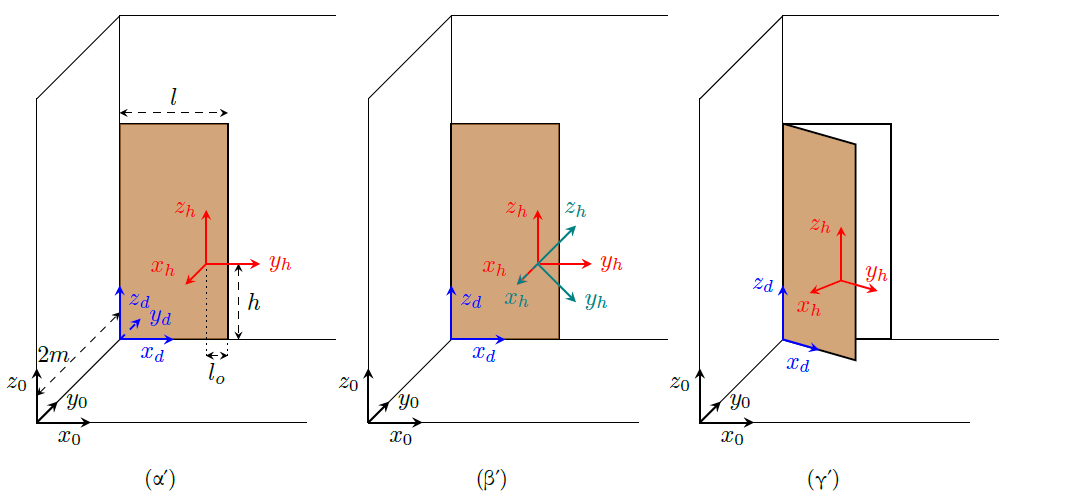
\includegraphics[width=1\linewidth]{plotsPartA/plot0_workplace.png}
    \caption{}
    \label{fig:plot0_workplace}
\end{figure}


\subsection{Περιγραφή στιγμιαίας θέσης και προσανατολισμού πλαισίων στον χρόνο}

Τα πλαίσια $\{D\}$ \& $\{H\}$ κινούνται σε σχέση με το αδρανειακό πλαίσιο $\{0\}$. 
Για να εκφράσουμε την στιγμιαία θέση και τον στιγμιαίο προσανατολισμό των πλαισίων αυτών σε σχέση με το σύστημα αναφοράς (αδρανειακό πλαίσιο $\{0\}$) 
θα χρειαστεί να υπολογίσουμε τους \textit{\textbf{ομογενείς μετασχηματισμούς}} $g_{0d}(t), g_{0h}(t) \in SE(3)$, 
όπου $g_{0d}(t) = \begin{bmatrix} R_{0d}(t) & p_{0d}(t) \\ 0 & 1\end{bmatrix}$ και
$g_{0h}(t) = \begin{bmatrix} R_{0h}(t) & p_{0h}(t) \\ 0 & 1\end{bmatrix}$, αντίστοιχα.

\newgeometry{
    top=2cm,
    bottom=2cm,
    left=2cm,
    right=2cm
}

Το άνυσμα θέσης της αρχής του πλαισίου $\{D\}$ στο αδρανειακό πλαίσιο $\{0\}$ είναι σταθερό κατά την διάρκεια όλης της κίνησης 
και ίσο με $p_{0d}(t) = \begin{bmatrix} 0 & 2 &0 \end{bmatrix} ^{\top} \in \mathbb{R}^3, \ \forall t \in [0, T]$.

Αρχικά, για $t = 0$, όπως είναι φανερό και από την πρώτη πόζα του Σχήματος~\ref{fig:plot0_workplace}, 
τα πλαίσια $\{D\}$ και $\{0\}$ έχουν τον ίδιο προσανατολισμό\textemdash δηλαδή $R_{0d}(t = 0) = I_{3 \times 3}$. 
Έπειτα, κατά την διάρκεια που η πόρτα ανοίγει, ο προσανατολισμός του $\{D\}$ προκύπτει από την στροφή του $\{0\}$ κατά γωνία $\theta$ γύρω από τον άξονα $z$, συνεπώς:
\begin{equation*}
    R_{0d} = Rot(z, \theta) = 
    \begin{bmatrix}
        c_\theta & -s_\theta & 0 \\
        s_\theta & c_\theta & 0 \\
        0 &         0      &  1
    \end{bmatrix},
\end{equation*}
όπου $c_\theta = \cos(\theta)$ και $s_\theta = \sin(\theta)$.

Άρα, από τα παραπάνω προκύπτει ότι:
\begin{equation} \label{eq:g_0d}
    g_{0d} = \begin{bmatrix} R_{0d} & p_{0d}  \\ 0 & 1\end{bmatrix} = 
    \begin{bmatrix} 
        c_\theta  &  -s_\theta  &  0  &  0  \\
        s_\theta  &  c_\theta   &  0  &  2  \\
        0         &  0          &  1  &  0  \\
        0         &  0          &  0  &  1  
    \end{bmatrix}.
\end{equation}

Θα υπολογίσουμε τώρα τον ομογενή μετασχηματισμό $g_{dh}$ του πλαισίου $\{H\}$ ως προς το $\{D\}$. 
Προφανώς το άνυσμα της αρχής του πλαισίου $\{H\}$ είναι ως προς το $\{D\}$ σταθερό καθ' όλη την διάρκεια της κίνησης 
(μιας και τα δύο πλαίσια  είναι προσαρτημένα στο ίδιο σώμα/πόρτα)
και ίσο με $p_{dh}(t) = \begin{bmatrix} l - lo & 0 & h \end{bmatrix}^{\top} \in \mathbb{R}^3, \ \forall t \in [0, T]$.

Ο δε προσανατολισμός του πλαισίου $\{H\}$ ως προς το $\{D\}$, για χρονική στιγμή $t$, 
προκύπτει από μία σειρά στροφών γύρω από τους άξονες του κινούμενου πλαισίου $\{H\}$ και άρα 
σχηματίζεται με τον κατά σειρά πολλαπλασιασμό από \textit{δεξιά} με τον πίνακα της αντίστοιχης βασικής στροφής. 

Πιο συγκεκριμένα, ο προσανατολισμός του πλαισίου $\{H\}$ έχει προκύψει από στροφή του $\{D\}$ κατά γωνία $-90^{\circ}$ γύρω από την άξονα $z$ 
και έπειτα κατά γωνία $\phi$ γύρω από τον \textbf{νέο} άξονα του $x$ (όπως φαίνεται και στην μεσαία εικόνα στο σχήμα~\ref{fig:plot0_workplace}, για την χρονική στιγμή όπου $\phi = -45^{\circ}$).

Σύμφωνα με τα παραπάνω προκύπτει ο πίνακας στροφής ως:
\begin{equation}\label{eq:Rdh}
        R_{dh} = Rot(z, -90^{\circ}) Rot(x, \phi) = 
    \begin{bmatrix}
        0        & 1       & 0 \\
        -1     & 0         & 0 \\
        0 &         0       &  1
    \end{bmatrix} \begin{bmatrix}
        1        & 0       & 0 \\
        0     & c_{\phi}         & -s_{\phi} \\
        0 &         s_{\phi}      &  c_{\phi}
    \end{bmatrix} = \begin{bmatrix}
        0    &  c_{\phi}  & -s_{\phi} \\
        -1   &  0         &  0    \\
        0    &  s_{\phi}  &  c_{\phi}
    \end{bmatrix}
    .
\end{equation}

Επομένως, από τα παραπάνω βγάζουμε:
\begin{equation} \label{eq:g_dh}
    g_{dh} = \begin{bmatrix} R_{dh} & p_{dh}  \\ 0 & 1\end{bmatrix} = 
    \begin{bmatrix} 
        0         &  c_{\phi}  & -s_{\phi}  &  l - l_o  \\
        -1        &  0         &  0         &  0  \\
        0         &  s_{\phi}  &  c_{\phi}  &  h  \\
        0         &  0         &  0         &  1  
    \end{bmatrix}.
\end{equation}

Από τις \eqref{eq:g_0d} και \eqref{eq:g_dh} μπορούμε τώρα να υπολογίσουμε τον ομογενή μετασχηματισμό $g_{0h}$ ως:
\begin{equation} \label{eq:g_0h}
    g_{0h} = g_{0d} g_{dh} = \begin{bmatrix} 
        c_\theta  &  -s_\theta  &  0  &  0  \\
        s_\theta  &  c_\theta   &  0  &  2  \\
        0         &  0          &  1  &  0  \\
        0         &  0          &  0  &  1  
    \end{bmatrix} \begin{bmatrix} 
        0         &  c_{\phi}  & -s_{\phi}  &  l - l_o  \\
        -1        &  0         &  0         &  0  \\
        0         &  s_{\phi}  &  c_{\phi}  &  h  \\
        0         &  0         &  0         &  1  
    \end{bmatrix} = \begin{bmatrix} 
        s_{\theta}  &  c_{\phi} c_{\theta}  & -c_{\theta} s_{\phi}   &  c_{\theta} (l - l_o)  \\
        -c_{\theta} &  c_{\phi} s_{\theta}  & -s_{\phi} s_{\theta}   &  s_{\theta} (l - l_o) + 2  \\
        0           &  s_{\phi}             &  c_{\phi}              &  h  \\
        0           &  0                    &  0                     &  1  
    \end{bmatrix}.
\end{equation} 

\begin{examplebox}{Σχόλιο}
    Οι γωνίες $\theta$ και $\phi$ αποτελούν συναρτήσεις του χρόνου και περιγράφουν τις μεταβλητές των αρθρώσεων του συστήματος που μελετάμε, $q = \begin{bmatrix} \theta & \phi \end{bmatrix} ^{\top} \in \mathbb{R}^2$.
    
    Στις σχέσεις \eqref{eq:g_0d} και \eqref{eq:g_0h} υπολογίστηκαν οι ομογενείς μετασχηματισμοί $g_{0d}(t)$ και $g_{0h}(t)$. 
    Αυτοί εξαρτώνται από τις παραπάνω γωνίες και μπορούν να εκφραστούν ως συναρτήσεις των μεταβλητών των αρθρώσεων $q$\textemdash 
    δηλαδή ως $g_{0d}(q), g_{0h}(q): Q \rightarrow SE(3)$,
    όπου $Q$ είναι ο χώρος των επιτρεπτών τιμών των αρθρώσεων.
\end{examplebox}

\subsection{Υπολογισμός Ταχυτήτων}

Στην παραπάνω ανάλυση υπολογίσαμε την τροχιά $g_{0h}(t)$ η οποία\textemdash όπως αναφέραμε ήδη\textemdash 
εκφράζει την στιγμιαία θέση και τον στιγμιαίο προσανατολισμό του $\{H\}$ σε σχέση με το αδρανειακό σύστημα αναφοράς. 

Μας ενδιαφέρει τώρα να υπολογίσουμε την σχετική κίνηση/ταχύτητα μεταξύ των πλαισίων. 
Αυτό θα μας χρησιμεύσει στο επόμενο βήμα ώστε να μπορέσουμε να βρούμε την Ιακωβιανή του άκρου.  
Θα υπολογίσουμε τώρα την ταχύτητα $V = \begin{bmatrix} v & \omega\end{bmatrix}^{\top} \in \mathbb{R}^{6}$, για καθένα από τα $\{D\}$ και $\{H\}$.

\begin{examplebox}{Συμβολισμός}
    Με τον συμβολισμό $^{C}V_{ab}$ θα αναφερόμαστε στο άνυσμα της ταχύτητας της κίνησης του $\{B\}$ ως προς το πλαίσιο $\{A\}$, \textit{\textbf{εκφρασμένο}} στις συντεταγμένες του πλαισίου $\{C\}$.
    Το $^{C}V_{ab}$ περιλαμβάνει τη \textit{μεταφορική ταχύτητα} της αρχής του $\{B\}$ \textbf{και} τη \textit{γωνιακή ταχύτητα} (ως προς το πλαίσιο $\{A\}$).
\end{examplebox}

Για το πλαίσιο $\{D\}$:
\begin{itemize}[nolistsep, noitemsep]
    \item Η μεταφορική ταχύτητα της αρχής του πλαισίου $\{D\}$, ως προς το πλαίσιο $\{0\}$, εκφρασμένη στις συντεταγμένες του ίδιου του πλαισίου $\{D\}$ είναι:
    \begin{equation}\label{eq:v0d_D}
        v_d = R_{0d}^{\top} \dot{p}_{0d} = \begin{bmatrix}
        c_\theta  & s_\theta & 0 \\
        -s_\theta & c_\theta & 0 \\
        0 &         0      &  1
    \end{bmatrix} \begin{bmatrix}
        0 \\
        0 \\
        0 
    \end{bmatrix} = \begin{bmatrix}
        0 \\
        0 \\
        0 
    \end{bmatrix},
    \end{equation}
    προφανές\textemdash μιας και η κίνηση του πλαισίου $\{D\}$ είναι \textit{αμιγώς περιστροφική} (δεν εκτελεί μεταφορική κίνηση σε σχέση με το πλαίσιο $\{0\}$).

    \item Η γωνιακή ταχύτητα σε συντεταγμένες και πάλι του ίδιου του πλαισίου $\{D\}$ είναι:
    \begin{equation}\label{eq:omegahatD}
        \widehat{\omega}_d = R_{0d}^{\top} \dot{R}_{0d} = 
        \begin{bmatrix}
            c_\theta  & s_\theta & 0 \\
            -s_\theta & c_\theta & 0 \\
            0 &         0      &  1
        \end{bmatrix} \begin{bmatrix}
            -s_\theta \dot\theta  &  -c_\theta \dot\theta &  0 \\
            c_\theta  \dot\theta &  -s_\theta  \dot\theta &  0 \\
            0          &  0          &  0
        \end{bmatrix} = \begin{bmatrix}
            0          &  -\dot\theta          &  0 \\
            \dot\theta          &  0           &  0 \\
            0          &  0           &  0
        \end{bmatrix}
        \in so(3),
    \end{equation}
    όπου με $\widehat{\omega}$ συμβολίζουμε τον αντισυμμετρικό πίνακα που αναπαριστά το $\omega \in \mathbb{R}^3$. Άρα:
    \begin{equation}\label{eq:omegaD}
        \omega_d = \begin{bmatrix}
            0  & 0  &  \dot\theta 
        \end{bmatrix}^{\top},
    \end{equation}
    το οποίο μπορούμε να επαληθεύσουμε και διαισθητικά αν σκεφτούμε ότι το πλαίσιο $\{D\}$ περιστρέφεται μόνο γύρω από τον άξονα του $z_d$\footnote{Για τα μοναδιαία διανύσματα  των αξόνων $z$ έχουμε ότι: $\bar{z}_d \parallel \bar{z}_0$ και ομόρροπα, $\forall t \in [0, T]$.} διαγράφοντας γωνία $\theta(t)$. 
    Αυτό σημαίνει ότι η γωνιακή του ταχύτητα είναι $\omega_d = d\theta / dt \cdot \bar{z}_d= \dot\theta(t) \bar{z}_d$.
\end{itemize}

Από τις \eqref{eq:v0d_D} και \eqref{eq:omegaD} μπορούμε να υπολογίσουμε την ταχύτητα (συστροφή/twist) 
\begin{equation}\label{eq:V0d_D}
    ^{D}V_{0d} = \begin{bmatrix} v_d & \omega_d\end{bmatrix}^{\top} =
    \begin{bmatrix} 0 & 0 & 0 & 0 & 0 & \dot\theta  \end{bmatrix}^{\top}
\end{equation}
που αναφέρεται στο πλαίσιο $\{D\}$ και είναι εκφρασμένη σε αυτό (όπως δηλώνουν οι δείκτες).

Η συστροφή αυτή μπορεί να εκφραστεί σε \textit{ομογενή μορφή} από τον πίνακα 
$\widehat{V}_d = \begin{bmatrix} 
\widehat{\omega}_d & v_d \\ 
0 & 0
\end{bmatrix} \in \mathbb{R}^{4 \times 4}$, 
ο οποίος εναλλακτικά θα μπορούσε να υπολογιστεί και ως εξής:
\begin{equation}\label{eq:Vhatd}
    \widehat{V}_d = \begin{bmatrix} 
\widehat{\omega}_d & v_d \\ 
0 & 0
\end{bmatrix} = 
g_{0d}^{-1} \dot{g}_{0d}.
\end{equation}

Αντίστοιχα για το πλαίσιο $\{H\}$ μπορούμε να υπολογίσουμε\textemdash 
ως προς το πλαίσιο $\{D\}$ και εκφρασμένα στις συντεταγμένες του ίδιου του $\{H\}$\textemdash τα:
\begin{itemize}[noitemsep, nolistsep]
    \item $v_h = R_{dh}^{\top} \dot{p}_{dh}$ \\
    Το άνυσμα της θέσης, $p_{dh}$, του $\{H\}$ είναι ως προς το $\{D\}$ σταθερό και επομένως η παράγωγός του θα επιστρέψει ένα μηδενικό άνυσμα. 
    Συνεπώς, $v_h = \begin{bmatrix}
        0 &
        0 &
        0 
    \end{bmatrix}^{\top}$.
    
    \item $\widehat{\omega}_h = R_{dh}^{\top} \dot{R}_{dh}$ \\ 
    Η κίνηση του $\{H\}$ ως προς το $\{D\}$ είναι καθαρά περιστροφική και αν την εκφράσουμε στο σύστημα συντεταγμένων του $\{H\}$, εύκολα προκύπτει ότι:
    \begin{equation*}
        \omega_{h} = \dot\phi(t) \bar{x}_h \quad(\text{αν θέλαμε να το εκφράσουμε στο πλαίσιο $\{D\}$: } \,^{D}\omega_{h} = - \dot\phi(t) \bar{y}_d).
    \end{equation*}

    \begin{examplebox}{Παρατήρηση}
        Στο Σχήμα~\ref{fig:plot0_workplace} η μεσαία εικόνα, που δείχνει την περιστροφή του πόμολου γύρω από τον άξονα $\bar{x}_h$, έχει αρνητική φορά περιστροφής για το πλαίσιο $\{H\}$\textemdash δηλαδή ακολουθώντας τον κανόνα του δεξιού χεριού θα δούμε ότι το $\omega_{h}$ είναι ομόρροπο του $-\bar{x}_h$.
        Παρόλα αυτά, ορίσαμε τις γωνίες $\phi$ και $\theta$ να είναι θετικά ορισμένες. 
        Έπεται ότι όταν αναφερόμαστε σε $\phi = -45^{\circ}$ τότε εννοούμε την στροφή της πόζας που φαίνεται στο Σχήμα~\ref{fig:plot0_workplace}(β').
    \end{examplebox}

    Το παραπάνω αποτέλεσμα μπορούμε να το επαληθεύσουμε κάνοντας τις πράξεις:
    \begin{equation}
        \widehat{\omega}_h = R_{dh}^{\top} \dot{R}_{dh} \overset{\eqref{eq:Rdh}}{=} 
        \begin{bmatrix}
            0          &  -1  &  0  \\
            c_{\phi}   &  0   &  s_{\phi}  \\
            -s_{\phi}  &  0   &  c_{\phi}
        \end{bmatrix}
        \begin{bmatrix}
            0    &  -s_{\phi}  & -c_{\phi} \\
            0    &  0         &  0    \\
            0    &  c_{\phi}  &  -s_{\phi}
        \end{bmatrix} \dot\phi = 
        \begin{bmatrix}
            0    &  0    &  0 \\
            0    &  0    &  -1    \\
            0    &  1    &  0
        \end{bmatrix} \dot\phi,
    \end{equation}
    απ' όπου προκύπτει και πάλι ότι:
    \begin{equation}\label{eq:omegaH}
        \omega_h = \begin{bmatrix}
            \dot\phi  & 0  &  0
        \end{bmatrix}^{\top}.
    \end{equation}
    
\end{itemize}

Έτσι λοιπόν βρίσκουμε το: 
\begin{equation}\label{eq:Vdh_H}
    ^{H}V_{dh} = \begin{bmatrix} v_h & \omega_h\end{bmatrix}^{\top} = \begin{bmatrix} 0 & 0 & 0 & \dot\phi & 0 & 0 \end{bmatrix}^{\top}.
\end{equation}


\subsection{Ιακωβιανή του Άκρου $\{H\}$}
Ο υπολογισμός της Ιακωβιανής του άκρου $\{H\}$ είναι απαραίτητος, καθώς στην εκφώνηση δίνονται οι επιθυμητές τιμές ταχύτητας (και επιτάχυνσης) του άκρου, τόσο στην αρχική όσο και στην τελική του θέση. 
Από αυτές τις τιμές, στοχεύουμε στον υπολογισμό των αντίστοιχων επιθυμητών ταχυτήτων (και επιταχύνσεων) των μεταβλητών των αρθρώσεων για τις θέσεις αυτές.

% \begin{examplebox}{Ισοδυναμία Συστήματος με Σύστημα Ρομποτικού Βραχίωνα}
%     Στην ανάλυση που ως τώρα παρατέθηκε είναι εμφανές ότι γίνεται μια αντιστοιχία του συστήματος που μελετάμε με αυτό ενός ρομποτικού βραχίωνα. 
    
%     Συγκεκριμένα στο σύστημά μας, έχουμε δύο αρθρώσεις\textemdash μία στην πόρτα και μία στο πόμολο. 
%     Η άρθρωση της πόρτας αντιστοιχεί σε περιστροφή γύρω από τον μεντεσέ, ενώ η άρθρωση του πόμολου επιτρέπει την περιστροφή του γύρω από τον άξονά του.

%     Αυτή η διάταξη είναι ισοδύναμη με έναν ρομποτικό βραχίονα δύο βαθμών ελευθερίας. 
%     Έτσι, μπορούν να εφαρμοστούν οι ίδιες κινηματικές σχέσεις και μεθοδολογίες ανάλυσης.
% \end{examplebox}

Η ταχύτητα του πλαισίου $\{H\}$ (του "άκρου"/πόμολου) οφείλεται στην ταχύτητα των αρθρώσεων.
Άρα, μπορεί να βρεθεί από το άθροισμα των επιμέρους σχετικών συστροφών των συνδέσμων μεταξύ τους\textemdash 
με την προϋπόθεση ότι αυτές έχουν εκφραστεί στο πλαίσιο του άκρου, $\{H\}$.

Μας ενδιαφέρει να υπολογίσουμε το $^{H}V_{0h}$\textemdash δηλαδή την ταχύτητα του άκρου $\{H\}$ ως προς το πλαίσιο αναφοράς $\{0\}$ (αδρανειακό πλαίσιο) εκφρασμένη στο $\{H\}$\textemdash για να καταλήξουμε σε μία σχέση της μορφής:
\begin{equation}\label{eq:Jh}
    ^{H}V_{0h} = J_{h}(q) \dot{q},
\end{equation}
όπου $J_{h}(q) \in \mathbb{R}^{6 \times 2}$ θα είναι η Ιακωβιανή του άκρου του και $q$ οι μεταβλητές των αρθρώσεων του συστήματος που μελετάμε\footnote{
Συγκεκριμένα στο σύστημά μας, έχουμε δύο αρθρώσεις\textemdash μία στην πόρτα και μία στο πόμολο.
Η άρθρωση της πόρτας αντιστοιχεί σε περιστροφή γύρω από τον μεντεσέ, ενώ η άρθρωση του πόμολου επιτρέπει την περιστροφή του γύρω από τον άξονά του.
}, 
$q = \begin{bmatrix} \theta & \phi \end{bmatrix} ^{\top} \in \mathbb{R}^2$.

Ένας τρόπος υπολογισμού αυτής της ταχύτητας είναι μέσω σύνθεσης συστροφών. 
Η σχετική ταχύτητα του $\{H\}$ ως προς το $\{D\}$ έχει υπολογιστεί και περιγράφεται από την \eqref{eq:Vdh_H}, 
όπως επίσης και η ταχύτητα της κίνησης του $\{D\}$ ως προς το $\{0\}$ που περιγράφεται από την \eqref{eq:V0d_D}.
Από την σύνθεση των παραπάνω συστροφών παίρνουμε:
\begin{equation}\label{eq:V0h_H}
    ^{H}V_{0h} =
    \Gamma_{hd} \, ^{D}V_{0d} + \, ^{H}V_{dh}, 
\end{equation}
όπου $\Gamma_{hd} = \Gamma^{-1}_{dh} = \begin{bmatrix}
    R_{dh}^{\top}  &  - R_{dh}^{\top} \widehat{p}_{dh} \\
    0              &  R_{dh}^{\top}
\end{bmatrix} \in \mathbb{R}^{6 \times 6}$. Εφόσον γνωρίζουμε το ${p}_{dh}$ και από τη \eqref{eq:Rdh} το $R_{dh}$, παίρνουμε:
\begin{equation*}
     R_{dh}^{\top} = \begin{bmatrix}
        0          &  -1  &  0        \\
        c_{\phi}   &  0   &  s_{\phi}  \\
        -s_{\phi}  &  0   &  c_{\phi}
    \end{bmatrix},
\end{equation*}
και
\begin{equation*}
    R_{dh}^{\top} \widehat{p}_{dh} = \begin{bmatrix}
        0          &  -1  &  0        \\
        c_{\phi}   &  0   &  s_{\phi}  \\
        -s_{\phi}  &  0   &  c_{\phi}
    \end{bmatrix} \begin{bmatrix}
        0   &  -h      &  0        \\
        h   &  0       &  -(l-l_o) \\
        0   &  l-l_o   &  0
    \end{bmatrix} = \begin{bmatrix}
        -h   &  0                                &  l-l_o \\
        0    &  s_{\phi}(l-l_o) - h c_{\phi}    &  0 \\
        0    &  h s_{\phi} + c_{\phi}(l-l_o)    &  0
    \end{bmatrix}.
\end{equation*}
Οπότε βγάζουμε:
\begin{equation}\label{eq:Ghd}
    \Gamma_{hd} = \Gamma^{-1}_{dh} = \begin{bmatrix}
        R_{dh}^{\top}  &  - R_{dh}^{\top} \widehat{p}_{dh} \\
        0              &  R_{dh}^{\top}
    \end{bmatrix} = \begin{bmatrix}
        0          &  -1  &  0         &  h          &  0                               &  -(l-l_o) \\
        c_{\phi}   &  0   &  s_{\phi}  &  0          &  -s_{\phi}(l-l_o) + h c_{\phi}    &  0 \\
        -s_{\phi}  &  0   &  c_{\phi}  &  0          &  -h s_{\phi} - c_{\phi}(l-l_o)   &  0 \\
        0          &  0   &  0         &  0          &  -1                              &  0         \\
        0          &  0   &  0         &  c_{\phi}   &  0                               &  s_{\phi} \\
        0          &  0   &  0         &  -s_{\phi}  &  0                               &  c_{\phi} 
    \end{bmatrix}
\end{equation}

Εν τέλει, αντικαθιστώντας στην \eqref{eq:V0h_H} το αποτέλεσμα της \eqref{eq:Ghd} καταλήγουμε:
\begin{equation}\label{eq:V0h_H_complete}
    ^{H}V_{0h} \overset{\eqref{eq:V0d_D}, \eqref{eq:Vdh_H}}{=} \Gamma^{-1}_{dh}
    \begin{bmatrix} 0 \\ 0 \\ 0 \\ 0 \\ 0 \\ 1 \end{bmatrix} \dot\theta + 
    \begin{bmatrix} 0 \\ 0 \\ 0 \\ 1 \\ 0 \\ 0 \end{bmatrix} \dot\phi = 
    \begin{bmatrix} -(l-l_o) \\ 0 \\ 0 \\ 0 \\ s_{\phi} \\ c_{\phi} \end{bmatrix} \dot\theta + 
    \begin{bmatrix} 0 \\ 0 \\ 0 \\ 1 \\ 0 \\ 0 \end{bmatrix} \dot\phi = 
    \begin{bmatrix}
        -(l-l_o) & 0 \\ 0 & 0 \\ 0 & 0 \\ 0 & 1 \\ s_{\phi} & 0 \\ c_{\phi} & 0
    \end{bmatrix} 
    \begin{bmatrix}
        \dot\theta \\ \dot\phi
    \end{bmatrix},
\end{equation}
και λαμβάνοντας υπόψιν την \eqref{eq:Jh} έχουμε την Ιακωβιανή του άκρου:
\begin{equation}\label{eq:Jh_matrix}
    J_h(q) = \begin{bmatrix}
        -(l-l_o) & 0 \\ 0 & 0 \\ 0 & 0 \\ 0 & 1 \\ s_{\phi} & 0 \\ c_{\phi} & 0
    \end{bmatrix} .
\end{equation}

\begin{examplebox}{Παρατηρήσεις}
    \begin{enumerate}[noitemsep, nolistsep]
        \item Από την \eqref{eq:V0h_H_complete} έχουμε ότι η μεταφορική ταχύτητα του πλαισίου $\{H\}$ ως προς το αδρανειακό πλαίσιο $\{0\}$
        (εκφρασμένη στις συντεταγμένες του $\{H\}$) ισούται με: 
        \begin{equation}\label{eq:v0h}
            v_{0h} = \begin{bmatrix} -(l-l_o) \dot\theta & 0 & 0 \end{bmatrix}^{\top}.
        \end{equation}
        Το αποτέλεσμα αυτό είναι και διαισθητικά λογικό, καθώς η \textit{αρχή} του πλαισίου $\{H\}$ κινείται σε κυκλική τροχιά γύρω από τον άξονα της 
        πόρτας\footnote{Ορίζεται από το μοναδιαίο διάνυσμα $\bar{z}_d$, με κέντρο την αρχή του πλαισίου $\{D\}$.}, 
        σε απόσταση $l-l_o$ από αυτόν και με γωνιακή ταχύτητα $\dot\theta(t)$\footnote{
        Για αρνητικό ρυθμό μεταβολής της γωνίας $\theta$ (από $0$ σε $-30^{\circ}$), 
        θα έχουμε $v_{0h}$ ομόρροπο του $\bar{x}_{h}$ και άρα η πόρτα θα ανοίξει όπως δείχνει το Σχήμα~\ref{fig:plot0_workplace}(γ').
        }.
        
        \item Από την πάνω σχέση για το $v_{0h}$ είναι φανερό ότι με δεδομένη την μεταφορική ταχύτητα μπορούμε να βρούμε το $\dot\theta$. 
        Άρα αν γνωρίζουμε και την γωνιακή ταχύτητα $\omega_{0h}$ μπορούμε να βρούμε και την $\dot\phi$, μιας και:
        \begin{equation}\label{eq:omega0h}
            \omega_{0h} = \begin{bmatrix} \dot\phi & s_\phi \dot\theta & c_\phi \dot\theta \end{bmatrix}^{\top}.
        \end{equation}

        Αυτό σημαίνει ότι δεδομένης μιας επιθυμητής ταχύτητας του άκρου, $^{H}V_{0h}$, μπορούμε να βρούμε τις επιθυμητές ταχύτητες των αρθρώσεων $\dot q$.
    \end{enumerate}
\end{examplebox}

Τις χρονικές στιγμές $t_0 = 0$ και $t_f = T = 5 \sec$ θέλουμε το πόμολο/πλαίσιο $\{H\}$ να έχει μηδενική ταχύτητα και επιτάχυνση. Άρα:
\begin{equation}\label{eq:conditions_equations}
    ^{H}V_{0h}(\tau) = 0_{6 \times 1}, \quad 
    ^{H}\dot{V}_{0h}(\tau) = \begin{bmatrix}
        \dot{v}_{0h}(\tau) \\
        \dot{\omega}_{0h}(\tau)
    \end{bmatrix} = \begin{bmatrix}
         0_{3 \times 1} \\
         0_{3 \times 1}
    \end{bmatrix}, \quad
    \forall \tau \in \{ t_0, t_f \},
\end{equation}
και λύνοντας το σύστημα αυτών των εξισώσεων ως προς τις $\dot\phi, \ddot\phi$ και $\dot\theta, \ddot\theta$, έχουμε για τις χρονικές στιγμές $t_0 = 0$ και $t_f = T = 5 \sec$ μοναδική λύση:
\begin{equation}\label{eq:conditions}
    \dot{q} = \begin{bmatrix}
        \dot\theta \\ \dot\phi
    \end{bmatrix} = \begin{bmatrix}
        0 \\ 0
    \end{bmatrix}, \quad
    \ddot{q} = \begin{bmatrix}
        \ddot\theta \\ \ddot\phi
    \end{bmatrix} = \begin{bmatrix}
        0 \\ 0
    \end{bmatrix}, \quad \text{δεδομένου ότι: } \phi(0) = \phi(T) = 0\ (\& \ \theta(0) = 0, \theta(T) = -\pi/6~\mathrm{rad}).
\end{equation}


\subsection{Σχεδίαση Πολυωνυμικής Τροχιάς}
Μας ενδιαφέρει η τροχιά του άκρου $\{H\}$ (δηλαδή του πόμολου της πόρτας).
Η κίνηση μπορεί να χωριστεί σε \textit{δύο στάδια}:
\begin{enumerate}[nolistsep, noitemsep]
    \item $t_0 = 0 $ έως $ t_1$: \\
    Το πρώτο στάδιο είναι αυτό στο οποίο καλούμαστε να στρέψουμε το πόμολο $\{H\}$ ώστε να είμαστε σε θέση να ανοίξουμε την πόρτα. 
    Σε αυτό, η γωνία $\theta$ παραμένει σταθερή και ίση με μηδέν, ενώ η μόνη γωνία που μεταβάλλεται είναι η $\phi$ από $0~\mathrm{rad}$ σε $-\pi /4~\mathrm{rad}$.
    Όταν φτάσουμε στην χρονική στιγμή $t_1$, όπου $\phi(t_1) = -\pi /4~\mathrm{rad}$, περνάμε στο δεύτερο στάδιο.
    \item $t_1 $ έως $ t_f = T = 5 \sec$: \\
    Σε αυτό το στάδιο της κίνησης εκτελούνται ταυτόχρονα δύο μεταβολές στις γωνίες. 
    Αφενός, η γωνία $\phi$ θέλουμε να επιστρέψει στην αρχική της τιμή, από $\phi(t_1) = -\pi /4~\mathrm{rad}$ σε $\phi(t_f) = 0~\mathrm{rad}$, ώστε το πλαίσιο $\{H\}$ να επανέλθει στον αρχικό του προσανατολισμό ως προς το $\{D\}$.
    Αφετέρου, για να ανοίξει η πόρτα στις επιθυμητές μοίρες, θέλουμε και η γωνία $\theta$ να αρχίσει να μεταβάλλεται, από $\theta(t_1) = 0~\mathrm{rad}$ σε $\theta(t_f) = -\pi/6~\mathrm{rad}$.
\end{enumerate}

Για το πρώτο στάδιο της κίνησης, έχουμε $\theta(t) = 0, \forall t\in [t_0, t_1]$ (και άρα $\dot\theta(t) = 0$ και $\ddot\theta(t) = 0$), 
ενώ για το $\phi(t)$ πρέπει να λάβουμε υπόψιν τους παραπάνω περιορισμούς για την τροχιά στο διάστημα $[t_0, t_1]$, αλλά και αυτούς της \eqref{eq:conditions}. 
Δεν υπάρχουν σαφείς περιορισμοί που να αφορούν την χρονική στιγμή $t_1$, όμως μπορούμε να την αντιμετωπίσουμε ως μια "τελική" θέση για το πρώτο στάδιο της κίνησης. 
Επομένως θα ισχύουν για αυτήν οι ίδιοι περιορισμοί που αφορούν την τελική ταχύτητα και επιτάχυνση (οπότε θα πρέπει: πρώτη και δεύτερη παράγωγος της $\phi$ ίση με μηδέν). 

Όλοι οι περιορισμοί της τροχιάς συνοψίζονται παρακάτω:
\begin{align}
    \phi(t_0) = 0,   \quad &\dot\phi(t_0) = 0, \quad \ddot\phi(t_0) = 0, \nonumber \\
    \phi(t_1) = -\pi/4, \quad &\dot\phi(t_1) = 0, \quad \ddot\phi(t_1) = 0. \label{eq:conditions_part1}
\end{align}

Επειδή έχουμε $6$ συνολικά περιορισμούς απαιτείται χρήση πολυωνύμου με συνολικά $6$ ανεξάρτητες παραμέτρους, ώστε να μπορούν να ικανοποιούνται όλοι οι περιορισμοί. 
Επιλέγουμε ένα πολυώνυμο πέμπτης τάξης της μορφής:
\begin{align}
    &\phi(t) = k_0 + k_1 t + k_2 t^2 + k_3 t^3 + k_4 t^4 + k_5 t^5, \label{eq:phi_1} \\
    \text{με:} \nonumber \\
    &\dot\phi(t) = k_1 + 2 k_2 t + 3 k_3 t^2 + 4 k_4 t^3 + 5 k_5 t^4, \nonumber \\
    &\ddot\phi(t) = 2 k_2 + 6 k_3 t + 12 k_4 t^2 + 20 k_5 t^3, \nonumber
\end{align}

Αντικαθιστώντας την \eqref{eq:phi_1} και τις παραγώγους της στους περιορισμούς \eqref{eq:conditions_part1} καταλήγουμε στο $6 \times 6$ σύστημα εξισώσεων:
\begin{equation}\label{eq:system_1}
    \begin{bmatrix}
        1 & t_0 & t_0^2 & t_0^3   & t_0^4    & t_0^5    \\
        0 & 1   & 2 t_0 & 3 t_0^2 & 4 t_0^3  & 5 t_0^4  \\
        0 & 0   & 2     & 6 t_0^2 & 12 t_0^2 & 20 t_0^3 \\ 
        1 & t_1 & t_1^2 & t_1^3   & t_1^4    & t_1^5    \\
        0 & 1   & 2 t_1 & 3 t_1^2 & 4 t_1^3  & 5 t_1^4  \\
        0 & 0   & 2     & 6 t_1   & 12 t_1^2 & 20 t_1^3
    \end{bmatrix} \begin{bmatrix}
        k_0 \\ k_1 \\ k_2 \\ k_3 \\ k_4 \\ k_5
    \end{bmatrix} = \begin{bmatrix}
        0 \\ 0 \\ 0 \\ - \pi / 4 \\ 0 \\ 0
    \end{bmatrix},
\end{equation}
το οποίο έχει μοναδική λύση όταν $t_0 \neq t_1$, καθώς η ορίζουσα του $6 \times 6$ πίνακα είναι $-4(t_0 - t_1)^9$. 
Ο υπολογισμός και η απλοποίηση της ορίζουσας έγιναν στο MATLAB και παρατίθενται στο αρχείο \textit{detCalcPartA.m}.

Σύμφωνα με τα προηγούμενα, λύνοντας το σύστημα της \eqref{eq:system_1} μπορούμε να βρούμε, μέσω της \eqref{eq:phi_1}, την $\phi(t)$ για το διάστημα $[t_0 =0,\  t_1]$. 
Για το διάστημα αυτό έχουμε $\theta(t) = 0$. 
Αντικαθιστώντας τις συναρτήσεις αυτές στις \eqref{eq:g_0h} και \eqref{eq:V0h_H_complete} μπορούμε να υπολογίσουμε για κάθε χρονική στιγμή στο διάστημα αυτό την τροχιά (σε αυτή την περίπτωση περιλαμβάνει μόνο αλλαγές προσανατολισμού) και το διάνυσμα της ταχύτητας (περιέχει μόνο μη μηδενική γωνιακή συνιστώσα) για το πλαίσιο $\{H\}$. 

Περνάμε τώρα στο δεύτερο στάδιο της κίνησης στο οποίο αρχίζει να ανοίγει η πόρτα. 
Το χρονικό διάστημα της κίνησης που μελετάμε είναι το $[t_1,\  t_f = T = 5 \sec]$.
Κάνοντας αντίστοιχη ανάλυση με πριν μπορούμε εύκολα να δούμε πως όλοι οι περιορισμοί που έχουμε τώρα είναι οι εξής:
\begin{align}
    &\left\{
    \begin{aligned}
        \phi(t_1) = -\pi/4, \quad \dot\phi(t_1) = 0, \quad \ddot\phi(t_1) = 0 \\
        \phi(t_f) = 0, \quad \dot\phi(t_f) = 0, \quad \ddot\phi(t_f) = 0
    \end{aligned},
    \right.
    &\left\{
    \begin{aligned}
        \theta(t_1) = 0, \quad \dot\theta(t_1) = 0, \quad \ddot\theta(t_1) = 0 \\
        \theta(t_f) = -\pi / 6, \quad \dot\theta(t_f) = 0, \quad \ddot\theta(t_f) = 0
    \end{aligned},
    \right.
    \label{eq:conditions_part2_theta}
\end{align}

Και πάλι για καθεμία μεταβλητή άρθρωσης έχουμε συνολικά 6 περιορισμούς, συνεπώς επιλέγουμε:
\begin{align}
    &\left\{
    \begin{aligned}
        &\phi(t) = a_0 + a_1 t + a_2 t^2 + a_3 t^3 + a_4 t^4 + a_5 t^5 \\
        \text{με:} \\
        &\dot\phi(t) = a_1 + 2 a_2 t + 3 a_3 t^2 + 4 a_4 t^3 + 5 a_5 t^4   \\
        &\ddot\phi(t) = 2 a_2 + 6 a_3 t + 12 a_4 t^2 + 20 a_5 t^3  
    \end{aligned},
    \right.
    &\left\{
    \begin{aligned}
        &\theta(t) = b_0 + b_1 t + b_2 t^2 + b_3 t^3 + b_4 t^4 + b_5 t^5 \\
    \text{με:}  \\
    &\dot\theta(t) = b_1 + 2 b_2 t + 3 b_3 t^2 + 4 b_4 t^3 + 5 b_5 t^4  \\
    &\ddot\theta(t) = 2 b_2 + 6 b_3 t + 12 b_4 t^2 + 20 b_5 t^3  
    \end{aligned},
    \right.
    \label{eq:phi_2}
\end{align}
απ' όπου προκύπτουν τα εξής δύο συστήματα (καθένα εκ των οποίων έχει μοναδική λύση καθώς $t_1 \neq t_f$):
\begin{align}
    &\left\{
    \begin{aligned}
       \begin{bmatrix}
        1 & t_1 & t_1^2 & t_1^3   & t_1^4    & t_1^5    \\
        0 & 1   & 2 t_1 & 3 t_1^2 & 4 t_1^3  & 5 t_1^4  \\
        0 & 0   & 2     & 6 t_1^2 & 12 t_1^2 & 20 t_1^3 \\ 
        1 & t_f & t_f^2 & t_f^3   & t_f^4    & t_f^5    \\
        0 & 1   & 2 t_f & 3 t_f^2 & 4 t_f^3  & 5 t_f^4  \\
        0 & 0   & 2     & 6 t_f   & 12 t_f^2 & 20 t_f^3
    \end{bmatrix} \begin{bmatrix}
        a_0 \\ a_1 \\ a_2 \\ a_3 \\ a_4 \\ a_5
    \end{bmatrix} = \begin{bmatrix}
        - \pi / 4 \\ 0 \\ 0 \\ 0 \\ 0 \\ 0
    \end{bmatrix},
    \end{aligned}
    \right.
    &\left\{
    \begin{aligned}
        \begin{bmatrix}
        1 & t_1 & t_1^2 & t_1^3   & t_1^4    & t_1^5    \\
        0 & 1   & 2 t_1 & 3 t_1^2 & 4 t_1^3  & 5 t_1^4  \\
        0 & 0   & 2     & 6 t_1^2 & 12 t_1^2 & 20 t_1^3 \\ 
        1 & t_f & t_f^2 & t_f^3   & t_f^4    & t_f^5    \\
        0 & 1   & 2 t_f & 3 t_f^2 & 4 t_f^3  & 5 t_f^4  \\
        0 & 0   & 2     & 6 t_f   & 12 t_f^2 & 20 t_f^3
    \end{bmatrix} \begin{bmatrix}
        b_0 \\ b_1 \\ b_2 \\ b_3 \\ b_4 \\ b_5
    \end{bmatrix} = \begin{bmatrix}
        0 \\ 0 \\ 0 \\ - \pi / 6 \\ 0 \\ 0
    \end{bmatrix}.
    \end{aligned}
    \right.
    \label{eq:system_2}
\end{align}

Έτσι, λύνοντας τα συστήματα της \eqref{eq:system_2}, μπορούμε να υπολογίσουμε τις $\phi(t)$ και $\theta(t)$ για το διάστημα $[t_1, \ t_f]$.
Έπειτα, αντικαθιστώντας τις συναρτήσεις αυτές στις \eqref{eq:g_0h} και \eqref{eq:V0h_H_complete} μπορούμε να υπολογίσουμε για κάθε χρονική στιγμή στο διάστημα αυτό την τροχιά και το διάνυσμα της ταχύτητας για το πλαίσιο $\{H\}$, αντίστοιχα.

\begin{examplebox}{Σχόλια}
    \begin{enumerate}
        \item Η επιλογή μεταξύ των πολυωνύμων \eqref{eq:phi_1} και \eqref{eq:phi_2} για τη συνάρτηση $\phi(t)$ εξαρτάται από τη χρονική στιγμή $t$, καθώς κάθε πολυώνυμο περιγράφει διαφορετικό τμήμα της συνολικής κίνησης (αντίστοιχα για τη $\theta(t)$).
        Στην υλοποίησή μας στο MATLAB, όπως θα δούμε, είμαστε ιδιαίτερα προσεκτικοί ώστε να επιλέγουμε κάθε φορά τον σωστό κλάδο.

        \item Με την επιλογή $\dot{q} = 0$ και $\ddot{q} = 0$ τόσο στην αρχική όσο και στην τελική θέση κάθε σταδίου της κίνησης, 
        εξασφαλίζουμε ότι το πόμολο $\{H\}$ ξεκινά με και καταλήγει σε μηδενική ταχύτητα και επιτάχυνση 
        (όπως αναλύθηκε και στην ενότητα [1.3] για την Ιακωβιανή του άκρου). 
        Με την επιλογή μηδενικής ταχύτητας και επιτάχυνσης για την ενδιάμεση χρονική στιγμή $t_1$, 
        διατηρούμε τη συνοχή μεταξύ των επιμέρους σταδίων της κίνησης και την ομαλή μετάβαση μεταξύ αυτών.
    \end{enumerate}
\end{examplebox}


\newpage

\newgeometry{
    top=2cm,
    bottom=2cm,
    left=2cm,
    right=2cm
}

\section{Τμήμα Α - Αποτελέσματα MATLAB και Συμπεράσματα}
Στο αρχείο \textit{main.m} περιέχεται ο εκτελέσιμος κώδικας σε MATLAB για όλη την εργασία (Μέρη Α και Β).
Έχει χωριστεί σε μικρά sections για να είναι εύκολα αναγνώσιμος και έχουν εισαχθεί εντολές τύπου {\small \texttt{pause;}} ({\small \texttt{customPause(...)}}) 
για να επιτρέπεται η εύκολη προβολή των animation πριν προχωρήσει (με enter στο Command Window) στην επόμενη ομάδα από plots. 
Μπορούν να αγνοηθούν αυτόματα όλες οι εντολές παύσης αν θέσουμε {\small\texttt{debugMode = 1;}}.

Αρχικά λύνουμε καθένα από τα συστήματα \eqref{eq:system_1} και \eqref{eq:system_2}, για να βγάλουμε τις συναρτήσεις $\theta(t)$ και $\phi(t)$ στα δύο διαστήματα της κίνησης (όπως αναλύσαμε στην προηγούμενη ενότητα). 
Στο Σχήματα~\ref{fig:phi_t_logs} παραθέτουμε τα αποτελέσματα της επίλυσης των συστημάτων αυτών που αφορούν την άρθρωση $\phi(t)$ (αντίστοιχα στο Σχήμα~\ref{fig:theta_t_logs} για την $\theta(t)$).

Στα \ref{fig:phi_t} και \ref{fig:theta_t}, παραθέτουμε τις γραφικές παραστάσεις των $\theta(t)$ και $\phi(t)$ για όλο το διάστημα της κίνησης\textemdash όπως επίσης αυτές των παραγώγων τους. 
Από τις αναλυτικές εκφράσεις των πολυωνύμων για τα δύο διαστήματα, αλλά και από τις γραφικές παραστάσεις αυτών, παρατηρούμε πως οι τροχιές των αρθρώσεων που βρήκαμε είναι συνεχείς, με μηδενικές αρχικές και τελικές ταχύτητες και επιταχύνσεις για τις αρχικές και τελικές θέσεις. 

\begin{figure}[ht!]
    \centering
    \begin{minipage}{0.32\textwidth}
        \centering
        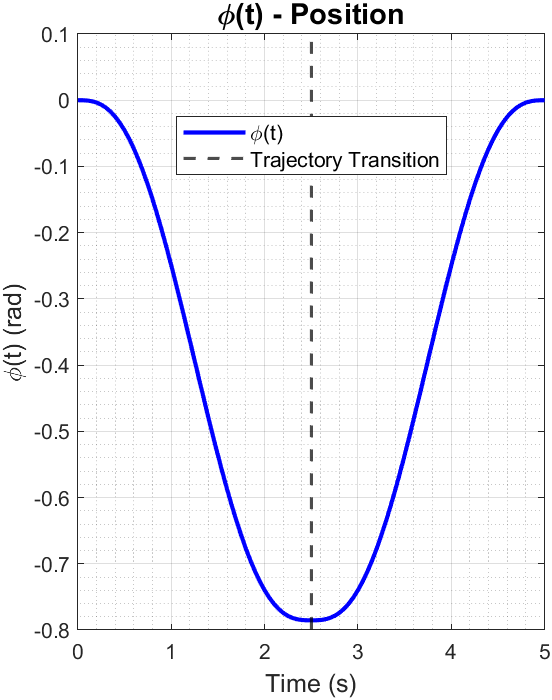
\includegraphics[width=0.99\linewidth]{plotsPartA/plot1_a_phi_t.png}
        % \caption{Image 1}
    \end{minipage}
    \hfill
    \begin{minipage}{0.32\textwidth}
        \centering
        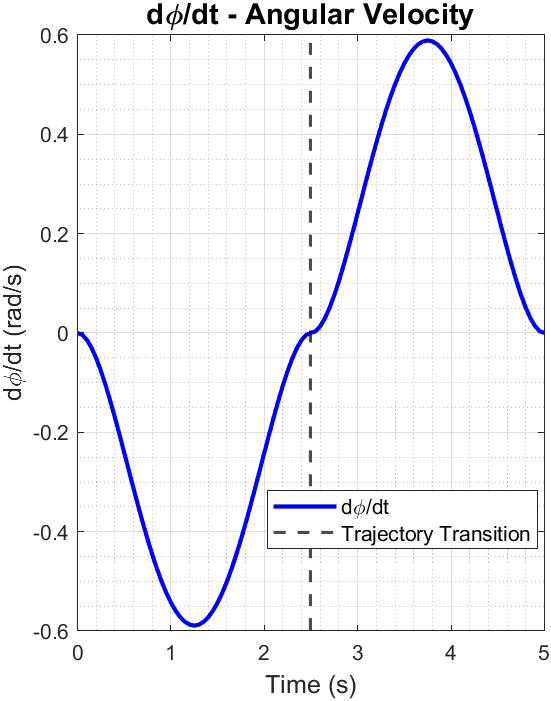
\includegraphics[width=0.99\linewidth]{plotsPartA/plot1_b_phi_dot_t.png}
        % \caption{Image 2}
    \end{minipage}
    \hfill
    \begin{minipage}{0.32\textwidth}
        \centering
        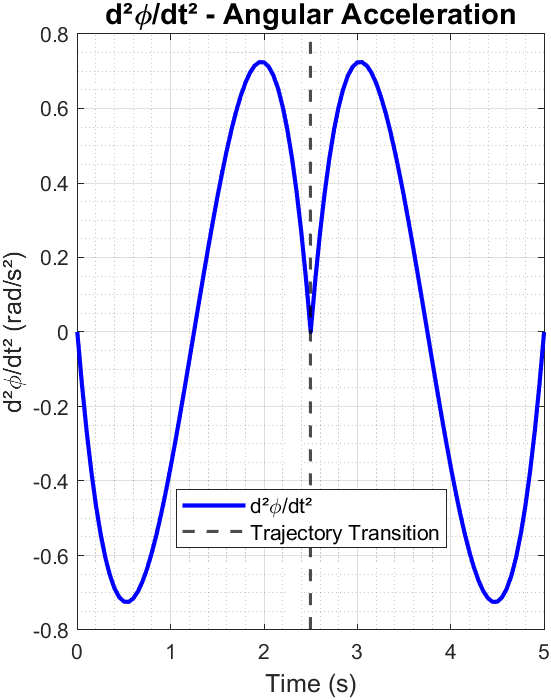
\includegraphics[width=0.99\linewidth]{plotsPartA/plot1_c_phi_ddot_t.png}
        % \caption{Image 3}
    \end{minipage}

    \caption{}
    \label{fig:phi_t}
\end{figure}

\textit{Σχόλια}:
\begin{itemize}[noitemsep, nolistsep]
    \item Η πρώτη γραφική παράσταση της \ref{fig:phi_t} είναι συμμετρική ως προς την ευθεία $t = t_1 = 2.5 \sec$, που είναι η στιγμή που αλλάζει το στάδιο της κίνησης. 
    Αυτό συμβαίνει επειδή τα δύο διαστήματα κίνησης έχουν ίδια χρονική περίοδο (ίση με $2.5 \sec$) και επειδή η κίνηση στο δεύτερο μισό είναι η αντίθετη της πρώτης. 
    Συνεπώς, εφόσον η περίοδος κίνησης στα δύο στάδια είναι ίδια, θα έχουμε το $\phi(t)$ να εκτελεί ακριβώς την αντίθετη με πριν κίνηση για να φτάσει εν τέλει στην αρχική του μηδενική τιμή. 
    
    \item Από τις γραφικές παραστάσεις θέσεων, ταχυτήτων και επιταχύνσεων είμαστε σε θέση να δούμε ότι όντως κάθε περιορισμός ικανοποιείται.  
\end{itemize}


\newpage

\newgeometry{
    top=1cm,
    bottom=2cm,
    left=2cm,
    right=2cm
}
 

\begin{figure}[ht!]
    \centering
    \begin{minipage}{0.98\textwidth}
        \centering
        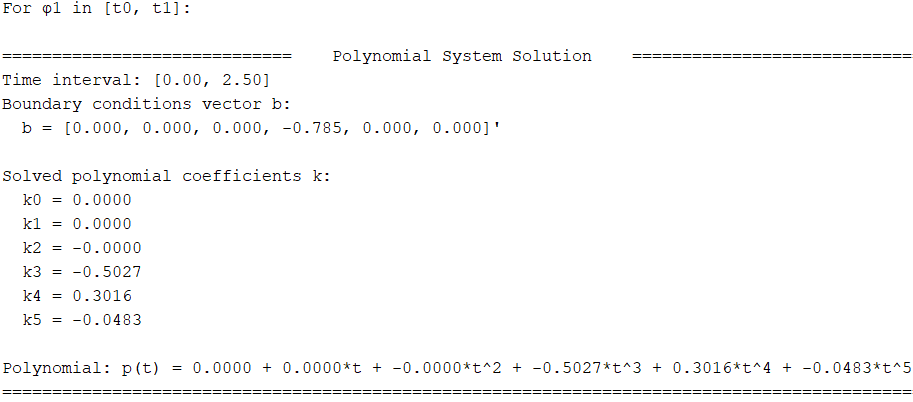
\includegraphics[width=0.53\linewidth]{plotsPartA/plot1_logs.png}
        % \caption{Image 1}
    \end{minipage}
    
    \vspace{1em} % Space between rows
    
    \begin{minipage}{0.98\textwidth}
        \centering
        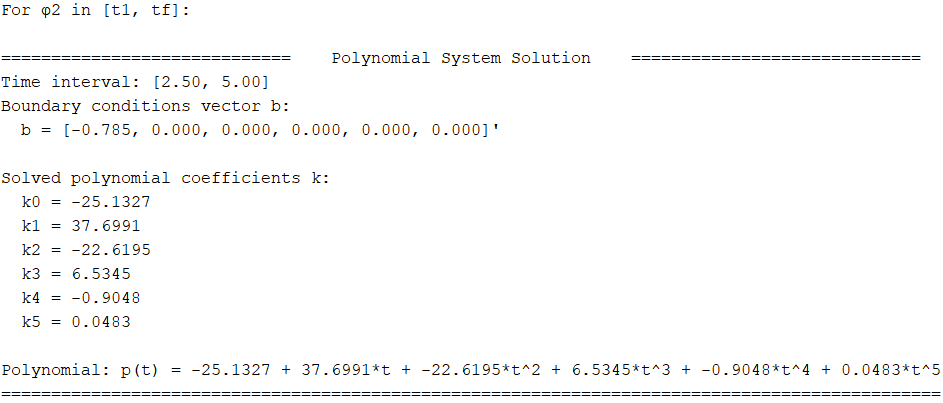
\includegraphics[width=0.53\linewidth]{plotsPartA/plot1_logs_2.png}
        % \caption{Image 2}
    \end{minipage}

    \caption{}
    \label{fig:phi_t_logs}
\end{figure}

\begin{figure}[ht!]
    \centering
    \begin{minipage}{0.32\textwidth}
        \centering
        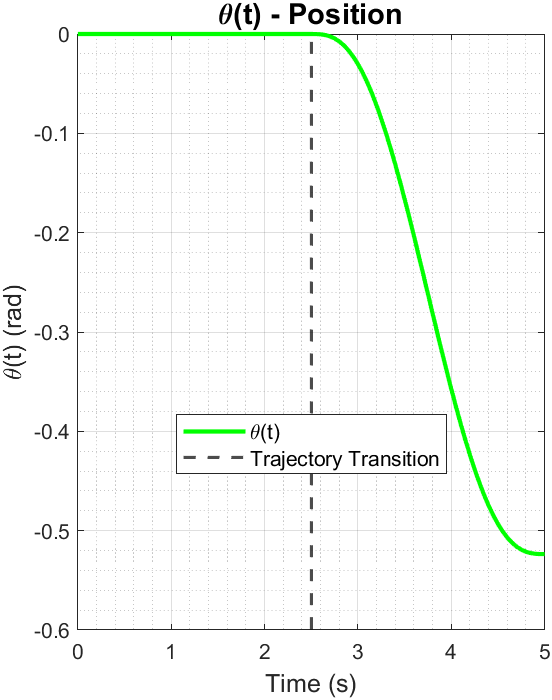
\includegraphics[width=0.99\linewidth]{plotsPartA/plot2_a_theta_t.png}
        % \caption{Image 1}
    \end{minipage}
    \hfill
    \begin{minipage}{0.32\textwidth}
        \centering
        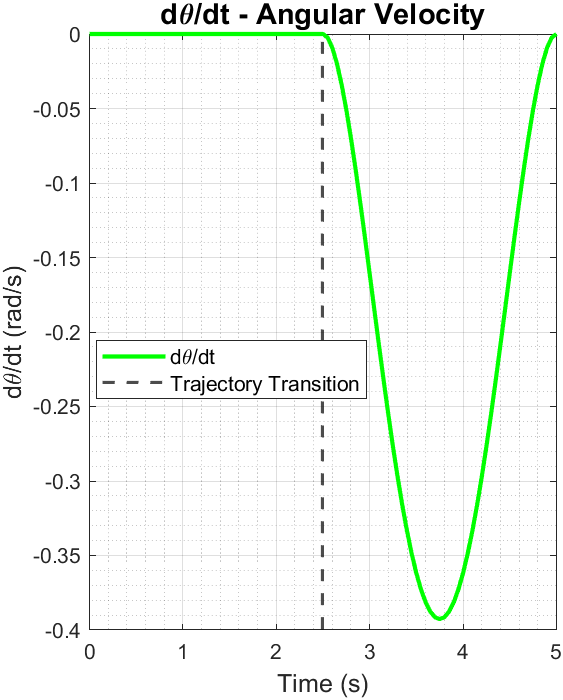
\includegraphics[width=0.99\linewidth]{plotsPartA/plot2_b_theta_dot_t.png}
        % \caption{Image 2}
    \end{minipage}
    \hfill
    \begin{minipage}{0.32\textwidth}
        \centering
        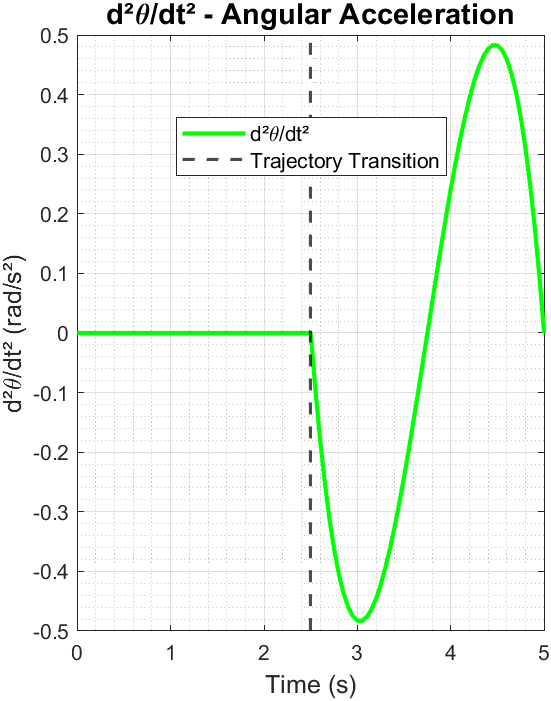
\includegraphics[width=0.99\linewidth]{plotsPartA/plot2_c_theta_ddot_t.png}
        % \caption{Image 3}
    \end{minipage}

    \caption{}
    \label{fig:theta_t}
\end{figure}

\begin{figure}[ht!]
    \centering
    \begin{minipage}{0.98\textwidth}
        \centering
        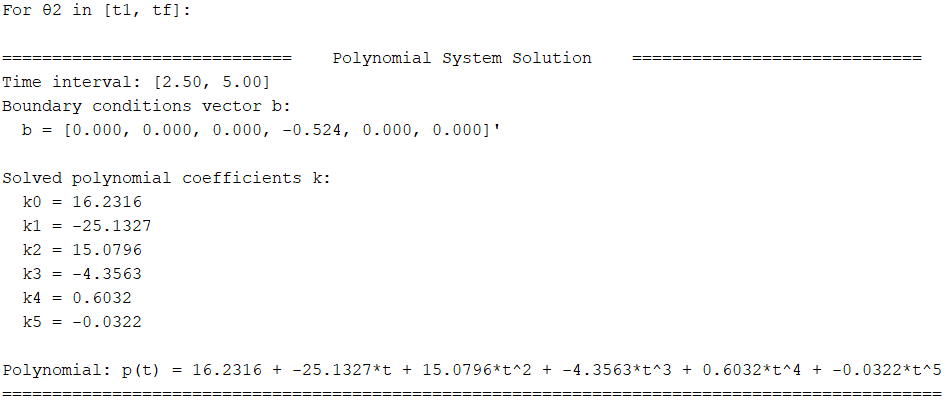
\includegraphics[width=0.53\linewidth]{plotsPartA/plot2_logs.png}
        % \caption{Image 1}
    \end{minipage}

    \caption{}
    \label{fig:theta_t_logs}
\end{figure}

\newpage
\newgeometry{
    top=2cm,
    bottom=2cm,
    left=2cm,
    right=2cm
}

Στις γραφικές παραστάσεις του Σχήματος~\ref{fig:vel_omega_1} παραθέτουμε την ταχύτητα (μεταφορική και γωνιακή) του πλαισίου $\{H\}$ ως προς το αδρανειακό πλαίσιο $\{0\}$ (όπως επίσης και τους ρυθμούς μεταβολής αυτών). 

\begin{examplebox}{Υπολογισμός του $\,^{0}V_{0h}$}
    Στην μαθηματική ανάλυση του προβλήματος υπολογίσαμε ήδη το $\,^{H}V_{0h}$, 
    που είναι το άνυσμα της ταχύτητας κίνησης του υπό μελέτη πλαισίου $\{H\}$ ως προς το αδρανειακό πλαίσιο $\{0\}$, \textit{εκφρασμένο} στις συντεταγμένες του $\{H\}$.
    Με τον υπολογισμό αυτού ήμασταν σε θέση να κατανοήσουμε και να ερμηνεύσουμε/επαληθεύσουμε ευκολότερα τα αποτελέσματα $v_{0h}$ και $\omega_{0h}$\textemdash μιας και αυτά ήταν εκφρασμένα στις συντεταγμένες του ίδιου του πλαισίου $\{H\}$.

    Στην συνέχεια, θα εκφράσουμε το άνυσμα αυτό στις συντεταγμένες του $\{0\}$ (υβριδική ταχύτητα). 
    Ο λόγος που το κάνουμε αυτό είναι επειδή θέλουμε στις γραφικές μας παραστάσεις να εκφράζουμε όλα τα διανύσματα ως προς ένα κοινό και αδρανειακό σύστημα συντεταγμένων (για συνοχή και σύγκριση). 

    Ισχύει ότι η γραμμική συνιστώσα της $\,^{0}V_{0h}$ αφορά της παράγωγο της θέσης της αρχής του πλαισίου $\{H\}$, 
    συνεπώς βρίσκεται από την:
    \begin{equation}\label{eq:v0h_0}
        \,^{0}v_{0h} = \dot{p}_{0h} = R_{0h} \,^{H}v_{0h},
    \end{equation}
    όπου τα $p_{0h}$ και $R_{0h}$ είναι γνωστά (καθώς έχουμε βρει τον ομογενή μετασχηματισμό $g_{0h}$ στην \eqref{eq:g_0h}) 
    και η $\,^{H}v_{0h} = v_{0h}$ είναι υπολογισμένη στην \eqref{eq:v0h}.
    
    
    Για την δε εύρεση της γωνιακής συνιστώσας της υβριδικής ταχύτητας (εκφρασμένης στο αδρανειακό πλαίσιο) μπορούμε είτε να την υπολογίσουμε από την
    $\,^{0}\widehat{\omega}_{0h} = \dot{R}_{0h} R_{0h}^{\top},$ είτε από την μετασχηματισμό:
    \begin{equation}\label{eq:omega0h_0}
        \,^{0}\omega_{0h} =  R_{0h} \,^{H}\omega_{0h},
    \end{equation}
    όπου η $\,^{H}\omega_{0h} = \omega_{0h}$ είναι υπολογισμένη στην \eqref{eq:omega0h}.
    \begin{center}
        \textit{Από τις \eqref{eq:v0h_0} και \eqref{eq:omega0h_0} μπορούμε να βρούμε την} $\,^{0}V_{0h}$.    
    \end{center}
\end{examplebox}

\begin{examplebox}{Μεταφορική και Γωνιακή Επιτάχυνση}
    Για το προς μελέτη πλαίσιο $\{H\}$ που κινείται σε σχέση με το αδρανειακό πλαίσιο $\{0\}$ θα βρούμε επίσης τα παρακάτω:
    \begin{itemize}[nolistsep, noitemsep]
        \item \textit{Μεταφορική επιτάχυνση (Translational acceleration)} της αρχής του πλαισίου $\{H\}$ ως προς το $\{0\}$:
        $$\ddot{p}_{0h} = \frac{d^2}{dt^2}p_{0h} = \frac{d}{dt} (\,^{0}v_{0h}),$$
        
        \item \textit{Γωνιακή επιτάχυνση (Angular acceleration)} του $\{H\}$ ως προς το $\{0\}$:
        $$\,^{0}\dot{\omega}_{0h} = \frac{d}{dt} (\,^{0}\omega_{0h}),$$
    \end{itemize}
    όπου και τα δύο (για λόγους συνοχής και σύγκρισης) έχουν εκφραστεί ως προς το αδρανειακό πλαίσιο.  
\end{examplebox}

\newpage
\newgeometry{
    top=2cm,
    bottom=2cm,
    left=2cm,
    right=2cm
}

\begin{figure}[ht!]
    \centering
    \begin{minipage}{0.48\textwidth}
        \centering
        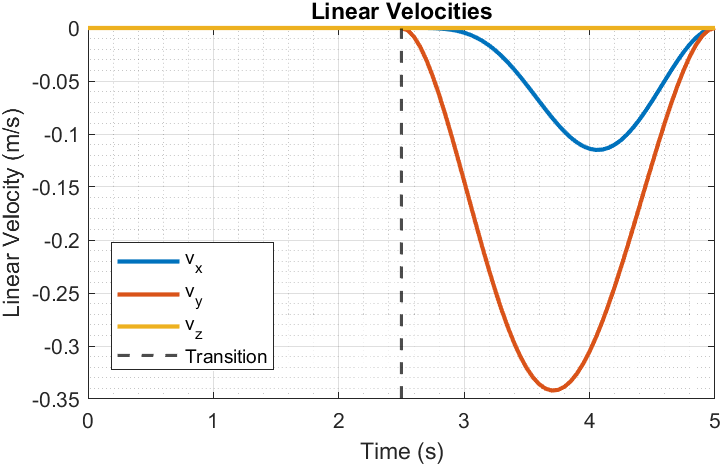
\includegraphics[width=0.9\linewidth]{plotsPartA/plot3_a_linear_velocity.png}
        % \caption{Image 1}
    \end{minipage}
    \hfill
    \begin{minipage}{0.48\textwidth}
        \centering
        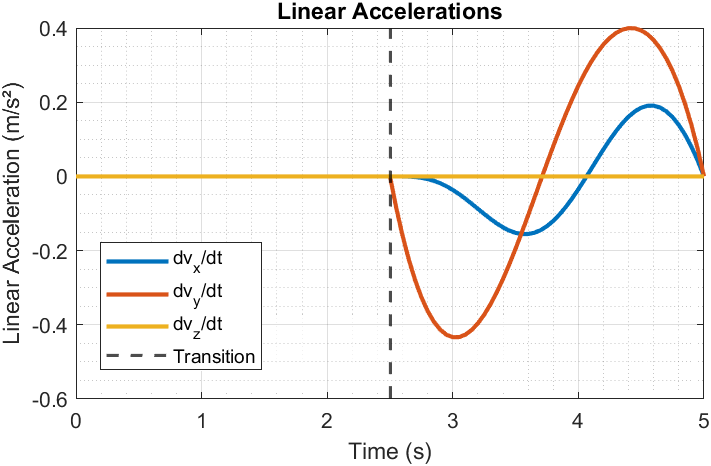
\includegraphics[width=0.9\linewidth]{plotsPartA/plot3_b_linear_accel.png}
        % \caption{Image 2}
    \end{minipage}
    
    \vspace{1em} % Space between rows
    
    \centering
    \begin{minipage}{0.48\textwidth}
        \centering
        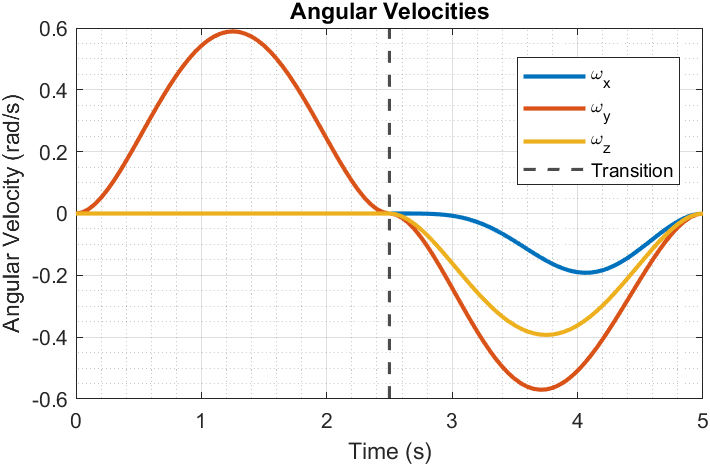
\includegraphics[width=0.9\linewidth]{plotsPartA/plot3_c_angular_vel.png}
        % \caption{Image 1}
    \end{minipage}
    \hfill
    \begin{minipage}{0.48\textwidth}
        \centering
        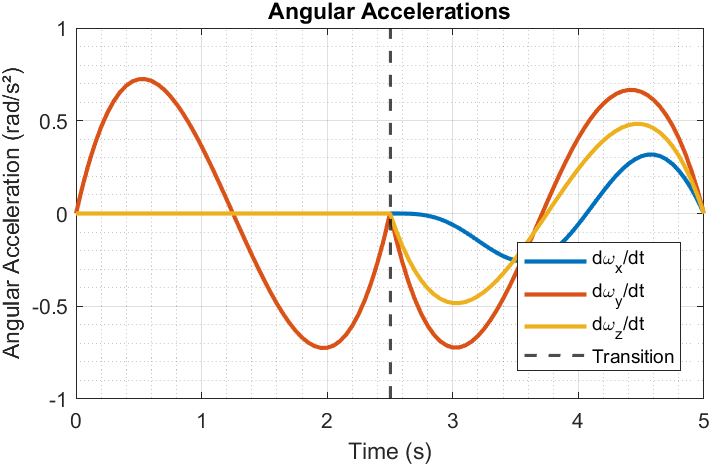
\includegraphics[width=0.9\linewidth]{plotsPartA/plot3_d_angular_accel.png}
        % \caption{Image 2}
    \end{minipage}

    \caption{}
    \label{fig:vel_omega_1}
\end{figure}

Για να επαληθεύσουμε ότι με τις συναρτήσεις των μεταβλητών των αρθρώσεων που βρήκαμε τα πλαίσια όντως βρίσκονται στις σωστές θέσεις και έχουν τον σωστό προσανατολισμό, σχεδιάσαμε και παραθέτουμε το Σχήμα \ref{fig:positions}.
Αυτό περιλαμβάνει τις πόζες για καθεμία από τις χρονικές στιγμές $t_0$, $t_1$ και $t_f$, όπως προκύπτουν από τους αντίστοιχους ομογενείς μετασχηματισμούς (ως προς το $\{0\}$). 

\begin{figure}[ht!]
    \centering
    \begin{minipage}{0.32\textwidth}
        \centering
        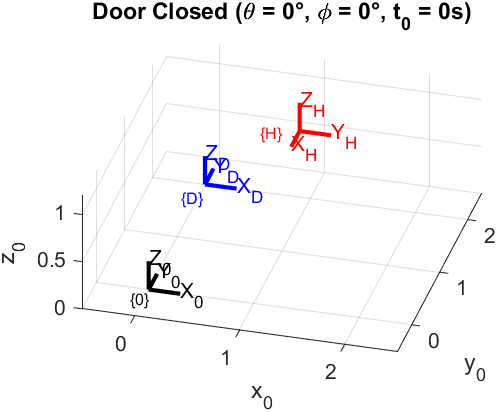
\includegraphics[width=0.99\linewidth]{plotsPartA/plot4_a_pose_door_closed.png}
        % \caption{Image 1}
    \end{minipage}
    \hfill
    \begin{minipage}{0.32\textwidth}
        \centering
        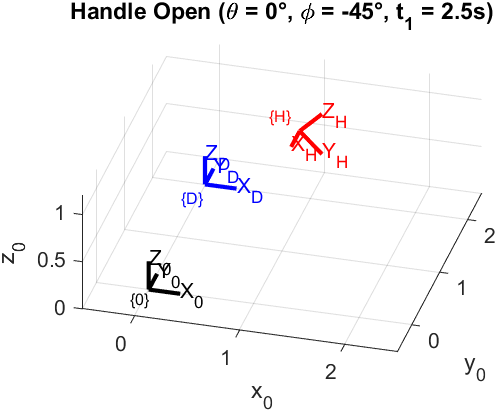
\includegraphics[width=0.99\linewidth]{plotsPartA/plot4_b_pose_handle_open.png}
        % \caption{Image 2}
    \end{minipage}
    \hfill
    \begin{minipage}{0.32\textwidth}
        \centering
        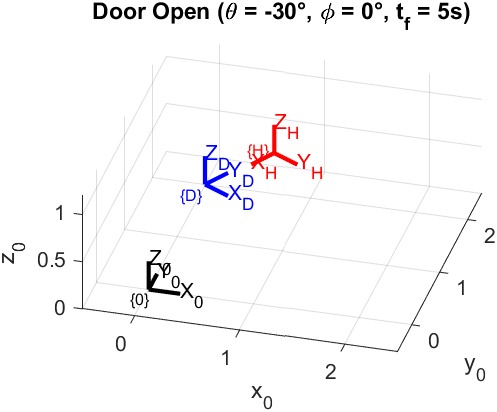
\includegraphics[width=0.99\linewidth]{plotsPartA/plot4_c_pose_door_open.png}
        % \caption{Image 1}
    \end{minipage}
    
    \caption{}
    \label{fig:positions}
\end{figure}

Τέλος, πριν περάσουμε στο Μέρος Β, παραθέτουμε τις τελευταίες ζητούμενες γραφικές παραστάσεις, στο Σχήμα~\ref{fig:Q}, που αναφέρονται στην τροχιά της θέσης της αρχής του πλαισίου $\{H\}$ (κάτω δεξιά) και του προσανατολισμού του πλαισίου $\{H\}$, πάντα ως προς το $\{0\}$.

Για την απεικόνιση της τροχιάς προσανατολισμού χρησιμοποιήσαμε Unit Quaternion. 
Στο πάνω αριστερά σχήμα, χαράξαμε την τροχιά του μοναδιαίου διανύσματος $\bar{k} \in \mathbb{R}^3$, το οποίο εκφράζει τον άξονα περιστροφής και 
στο δεξιά σχήμα έχουμε την γωνία $\theta_Q \in \mathbb{R}$ για κάθε χρονική στιγμή της κίνησης\textemdash 
όπως προκύπτουν από τον αντίστοιχο πίνακα στροφής $R_{0h}$, σύμφωνα με την δομή $Q = \begin{bmatrix}
    c_{\theta/2} \\ s_{\theta/2} \bar{k}
\end{bmatrix}$.

\begin{figure}[ht!]
    \centering
    \begin{minipage}{0.48\textwidth}
        \centering
        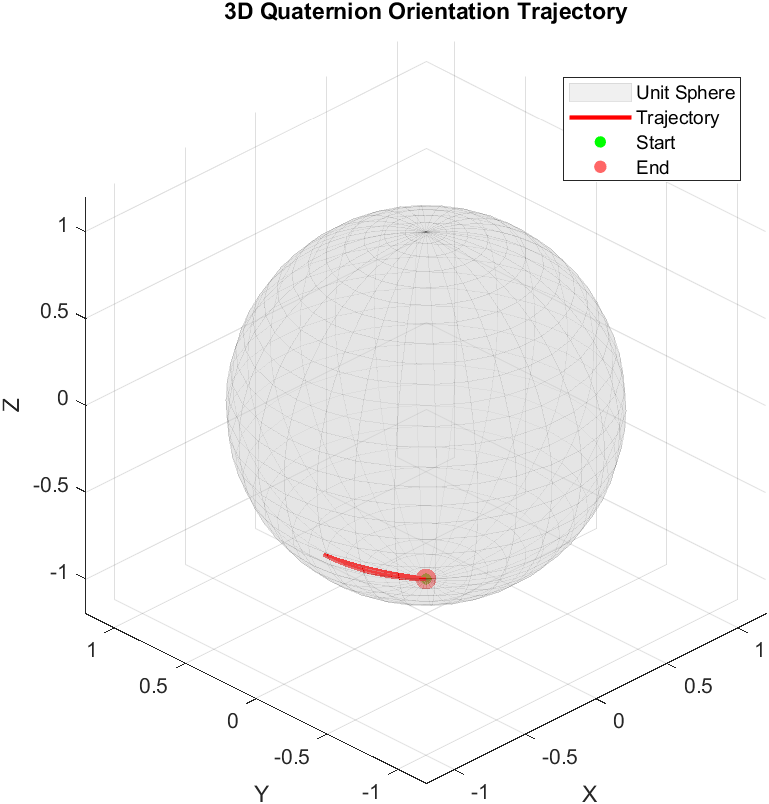
\includegraphics[width=0.8\linewidth]{plotsPartA/plot5_a_Q_vec.png}
        % \caption{Image 1}
    \end{minipage}
    \hfill
    \begin{minipage}{0.48\textwidth}
        \centering
        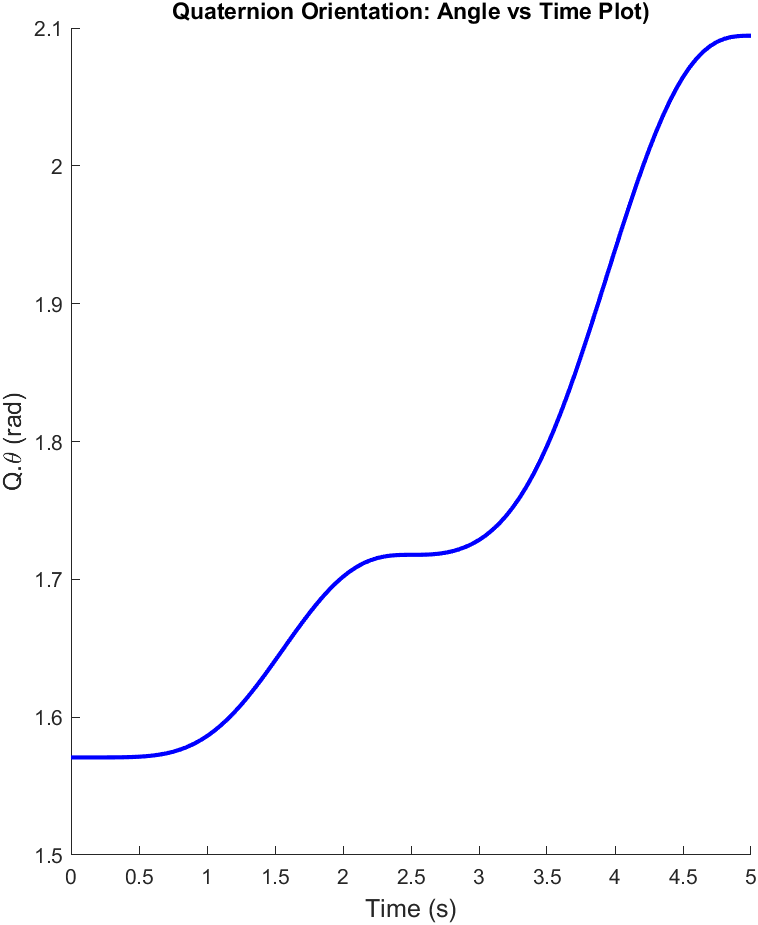
\includegraphics[width=0.7\linewidth]{plotsPartA/plot5_b_Q_time.png}
        % \caption{Image 2}
    \end{minipage}
    
    \vspace{1em} % Space between rows
    
    \centering
    \begin{minipage}{0.48\textwidth}
        \centering
        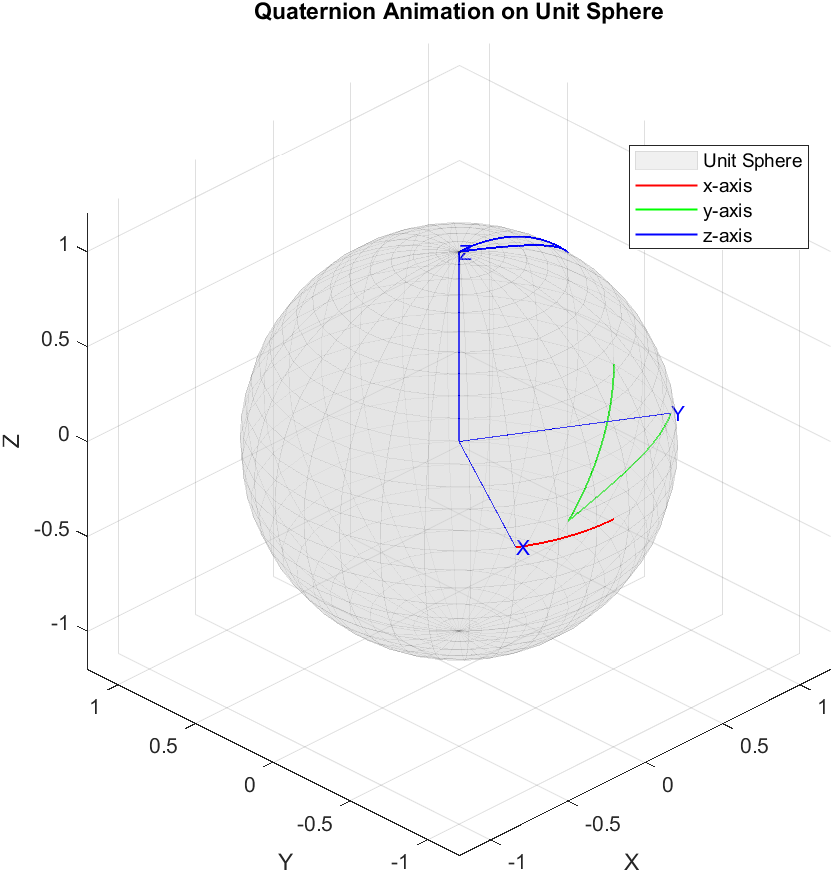
\includegraphics[width=0.8\linewidth]{plotsPartA/plot6_animate_rotation.png}
        % \caption{Image 1}
    \end{minipage}
    \hfill
    \begin{minipage}{0.48\textwidth}
        \centering
        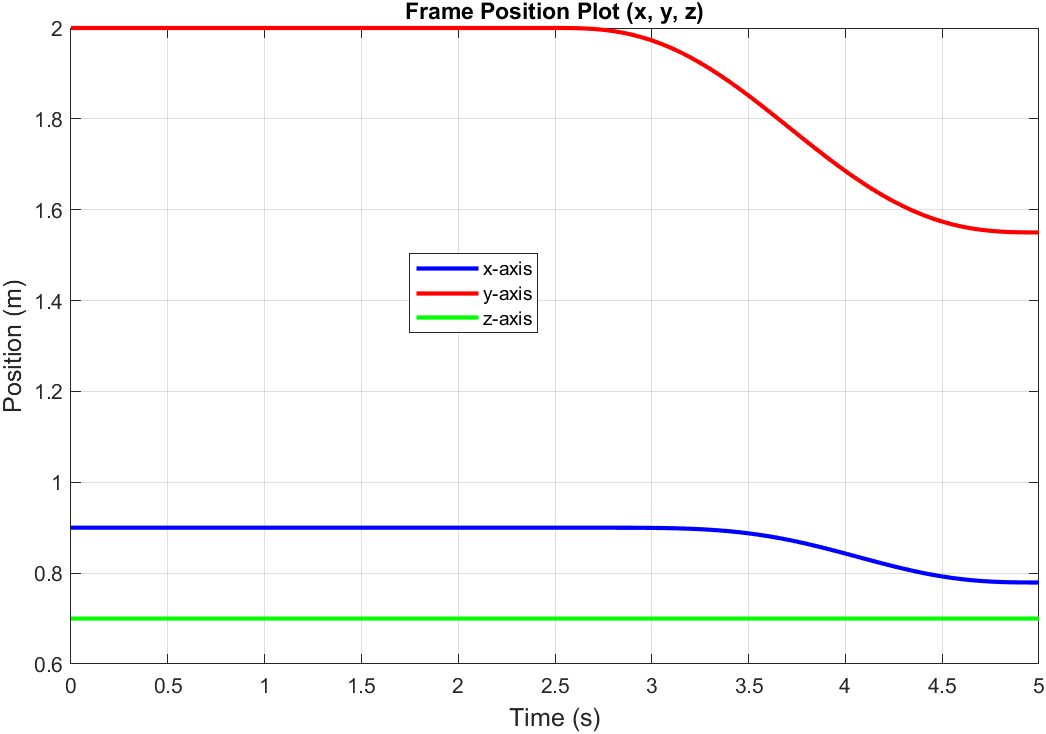
\includegraphics[width=1\linewidth]{plotsPartA/plot6_position_H.png}
        % \caption{Image 1}
    \end{minipage}
    
    \caption{}
    \label{fig:Q}
\end{figure}

\textit{Σχόλιο}: Το κάτω αριστερά σχήμα αποτελεί ένα animation της στροφής του πλαισίου $\{H\}$ στον χρόνο 
(εδώ παραθέτουμε μόνο την τελική του κατάσταση για την χρονική στιγμή $t_f$).

%%%%%%%%%%%%%%%%%%%%%%%%%%%%%%%%%%%%%%%%%%%%%%%%%%%%%%%%%%%% Part B %%%%%%%%%%%%%%%%%%%%%%%%%%%%%%%%%%%%%%%%%%%%%%%%%%%%%%%%%%%%%%%%%%%%
\newpage

\section{Τμήμα Β - Μαθηματική Ανάλυση}

\vspace{-\topsep}
\vspace{+2pt}
\begin{center}
    \textit{\textbf{Στόχος:} \\ 
    Σχεδίαση κατάλληλων εντολών ταχύτητας αρθρώσεων $\dot{q}_r \in \mathbb{R}^{6}$, \\
    ώστε το ρομπότ να κινήσει το πόμολο κατά τον τρόπο που σχεδιάστηκε στο Τμήμα Α, \\
    και να ανοίξει την πόρτα σε χρόνο $T = 5 \sec$ με περίοδο δειγματοληψίας $t_s = 0.01 \sec$.
    }
\end{center}

\begin{figure}[!ht]
    \centering
    \begin{subfigure}[b]{0.48\textwidth}
        \centering
        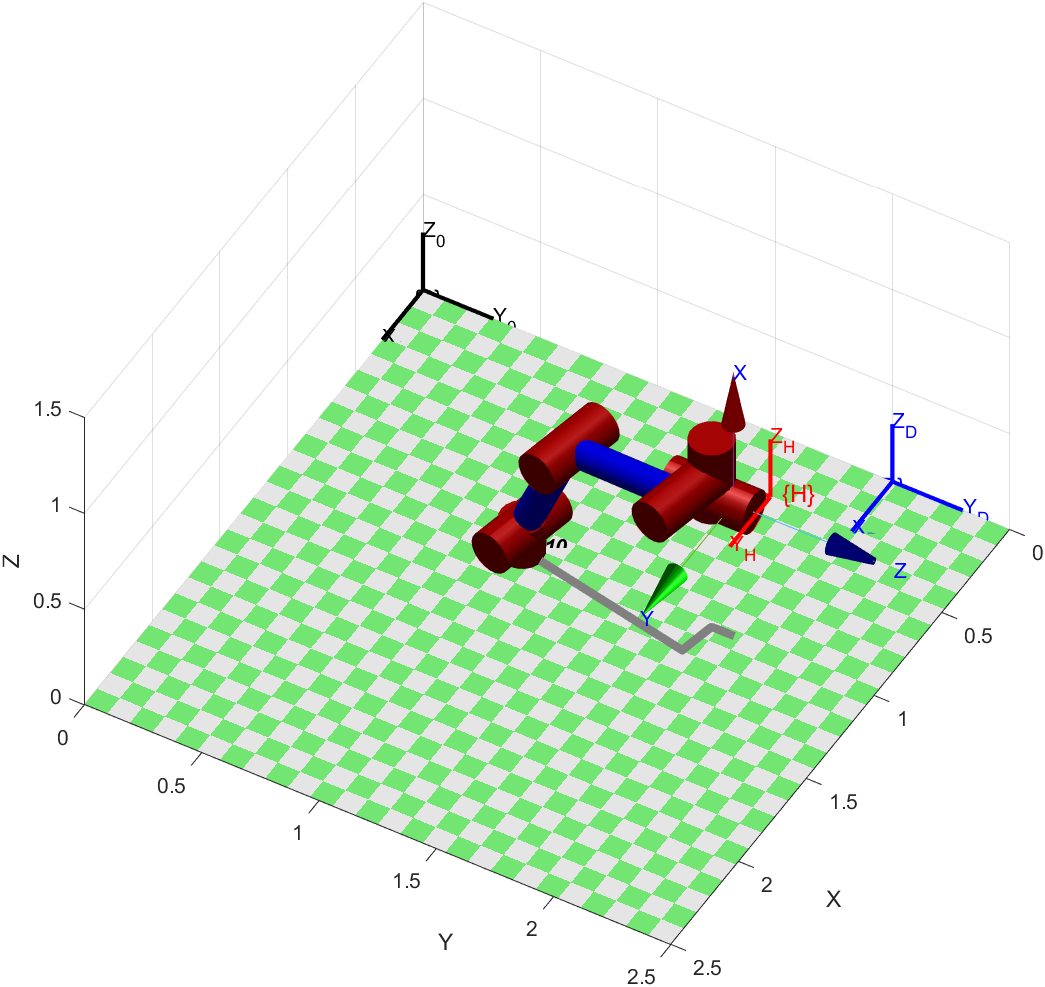
\includegraphics[width=\linewidth]{plotsPartB/plot1_a_robot_door_init.png}
        \caption{}
        \label{fig:plot1_a_robot_door_init}
    \end{subfigure}
    \hfill
    \begin{subfigure}[b]{0.48\textwidth}
        \centering
        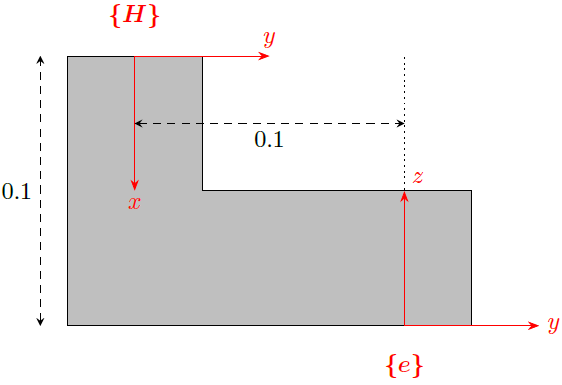
\includegraphics[width=\linewidth]{plotsPartB/plot1_b_robot_door.png}
        \caption{}
        \label{fig:plot1_b_robot_door}
    \end{subfigure}
    \caption{}
    \label{fig:plot1_workplace}
\end{figure}


\subsection{Περιγραφή στιγμιαίας θέσης και προσανατολισμού άκρου $\{e\}$}

Για να εκφράσουμε την στιγμιαία θέση και τον στιγμιαίο προσανατολισμό του πλαισίου $\{e\}$ σε σχέση με το σύστημα αναφοράς (αδρανειακό πλαίσιο $\{0\}$) 
θα χρειαστεί να υπολογίσουμε τον \textit{\textbf{ομογενή μετασχηματισμό}} $g_{0e}(t)\in SE(3)$, 
όπου $g_{0e}(t) = \begin{bmatrix} R_{0e}(t) & p_{0e}(t) \\ 0 & 1\end{bmatrix}$.

Για να το πετύχουμε αυτό θα υπολογίσουμε πρώτα τον $g_{he}$ του άκρου $\{e\}$ ως προς το πόμολο $\{H\}$. 
Σύμφωνα με την εκφώνηση πρέπει \textit{η σχετική πόζα του άκρου $\{e\}$ ως προς το πόμολο $\{H\}$ να είναι σταθερή $\forall t \in [t_0, t_f]$}. 
Άρα καθ' όλη την διάρκεια της κίνησης θα πρέπει να έχουμε $g_{he}$ σταθερό.

Από το Σχήμα~\ref{fig:plot1_b_robot_door} έχουμε:
\begin{equation}\label{eq:phe}
    p_{he}(t) = \begin{bmatrix} 0.1 & 0.1 & 0 \end{bmatrix}^{\top}.
\end{equation}
Επίσης ο προσανατολισμός του πλαισίου $\{e\}$ ως προς το $\{H\}$\textemdash που πρέπει να είναι επίσης χρονικά σταθερός\textemdash 
έχει προκύψει από μία στροφή του πλαισίου $\{H\}$ γύρω από τον άξονά του $\bar{y}_h$ (ομόρροπο του $\bar{y}_e)$ κατά γωνία $-90^{\circ}$, 
επομένως ισχύει:
\begin{equation}\label{eq:Rhe}
        R_{he} = Rot(y, -90^{\circ}) = \begin{bmatrix}
        0   &  0  &  -1  \\
        0   &  1  &  0   \\
        1   &  0  &  0
    \end{bmatrix},
\end{equation}
και, τελικά παίρνουμε τον πίνακα ομογενούς μετασχηματισμού:
\begin{equation} \label{eq:g_he}
    g_{he} = \begin{bmatrix} R_{he} & p_{he}  \\ 0 & 1\end{bmatrix} = 
    \begin{bmatrix} 
        0   &  0  & -1  &  0.1  \\
        0   &  1  &  0  &  0.1  \\
        1   &  0  &  0  &  0  \\
        0   &  0  &  0  &  1  
    \end{bmatrix}.
\end{equation}

Από τις \eqref{eq:g_he} και \eqref{eq:g_0h} μπορούμε τώρα να υπολογίσουμε τον ομογενή μετασχηματισμό $g_{0e}$ ως:
\begin{align} \label{eq:g_0e}
    g_{0e} = g_{0h} g_{he} = 
    \begin{bmatrix} 
        s_{\theta}  &  c_{\phi} c_{\theta}  & -c_{\theta} s_{\phi}   &  c_{\theta} (l - l_o)  \\
        -c_{\theta} &  c_{\phi} s_{\theta}  & -s_{\phi} s_{\theta}   &  s_{\theta} (l - l_o) + 2  \\
        0           &  s_{\phi}             &  c_{\phi}              &  h  \\
        0           &  0                    &  0                     &  1  
    \end{bmatrix} \begin{bmatrix} 
        0   &  0  & -1  &  0.1  \\
        0   &  1  &  0  &  0.1  \\
        1   &  0  &  0  &  0  \\
        0   &  0  &  0  &  1  
    \end{bmatrix} = \\
    \begin{bmatrix} 
        -c_{\theta} s_{\phi} & c_{\phi} c_{\theta} & -s_{\theta} & \frac{s_{\theta}}{10} + \frac{c_{\phi} c_{\theta}}{10} + c_{\theta}(l - l_o) \\
        -s_{\phi} s_{\theta} & c_{\phi} s_{\theta} & c_{\theta} & \frac{c_{\phi} s_{\theta}}{10} - \frac{c_{\theta}}{10} + s_{\theta}(l - l_o) + 2 \\
        c_{\phi} & s_{\phi} & 0 & h + \frac{s_{\phi}}{10} \\
        0 & 0 & 0 & 1
    \end{bmatrix}. \notag    
\end{align}
\textit{Σημείωση}: Η πράξη παρατίθεται για πληρότητα. Στο MATLAB εκτελούμε εκ νέου τον πολ/σμό.

Τέλος, πριν περάσουμε στην ανάλυση της ταχύτητας, θα εκφράσουμε επίσης την θέση του άκρου του ρομπότ ως προς την βάση του, $\{B\}$.
Η βάση αυτή έχει προσανατολισμό $R_{0b} = I_{3 \times 3}$ και βρίσκεται στην θέση 
$p_{0b} = \begin{bmatrix} 1 & 1 & 0 \end{bmatrix}^{\top}$\textemdash 
άρα ο $g_{0b}$ είναι γνωστός και ίσος με:
\begin{equation} \label{eq:g_0b}
    g_{0b} = \begin{bmatrix} R_{0b} & p_{0b}  \\ 0 & 1\end{bmatrix} = 
    \begin{bmatrix} 
        1   &  0  &  0  &  1  \\
        0   &  1  &  0  &  1  \\
        0   &  0  &  1  &  0  \\
        0   &  0  &  0  &  1  
    \end{bmatrix},
\end{equation}
όπως επίσης και αντίστροφός του, ο οποίος μπορεί να υπολογιστεί από την:
\begin{equation} \label{eq:g_b0}
    g_{b0} = g_{0b}^{-1}
    = \begin{bmatrix} R_{0b}^{\top} & - R_{0b}^{\top} p_{0b}  \\ 0 & 1\end{bmatrix} = 
    \begin{bmatrix} 
        1   &  0  &  0  &  -1  \\
        0   &  1  &  0  &  -1  \\
        0   &  0  &  1  &  0  \\
        0   &  0  &  0  &  1  
    \end{bmatrix}.
\end{equation}

Έτσι, από τις \eqref{eq:g_0e} και \eqref{eq:g_b0} προκύπτει το ζητούμενο:
\begin{equation} \label{eq:g_be}
    g_{be} = g_{b0} g_{0e} = \begin{bmatrix} 
        -c_{\theta} s_{\phi} & c_{\phi} c_{\theta} & -s_{\theta} & \frac{s_{\theta}}{10} + \frac{c_{\phi} c_{\theta}}{10} + c_{\theta}(l - l_o) - 1 \\
        -s_{\phi} s_{\theta} & c_{\phi} s_{\theta} & c_{\theta} & \frac{c_{\phi} s_{\theta}}{10} - \frac{c_{\theta}}{10} + s_{\theta}(l - l_o) + 1 \\
        c_{\phi} & s_{\phi} & 0 & h + \frac{s_{\phi}}{10} \\
        0 & 0 & 0 & 1
    \end{bmatrix}.
\end{equation} 

\begin{examplebox}{Εναλλακτικός Τρόπος Υπολογισμού $g_{be}$}
    Δεδομένου ότι το πλαίσιο $\{B\}$ έχει τον \textit{ίδιο προσανατολισμό} με το πλαίσιο αναφοράς $\{0\}$, 
    το μόνο που αλλάζει από την \eqref{eq:g_0e} στην \eqref{eq:g_be} είναι η έκφραση του ανύσματος θέσης $p$,
    για το οποίο έχουμε $p_{be} = p_{0e} - p_{0b}$.
\end{examplebox}


\subsection{Υπολογισμός Ταχύτητας Άκρου $\{e\}$}
Στην παραπάνω ανάλυση για το άκρο $\{e\}$ υπολογίσαμε την τροχιά $g_{0e}(t)$ ως προς το πλαίσιο αναφοράς $\{0\}$ και την $g_{be}(t)$ ως προς το πλαίσιο της βάσης $\{B\}$.
Μας ενδιαφέρει τώρα να υπολογίσουμε το άνυσμα της ταχύτητας του άκρου $\{e\}$ ως προς την σταθερή βάση του $\{B\}$,  
δηλαδή την ταχύτητα $\,^{e}V_{be} = \begin{bmatrix} \,^{e}v_{be} & \,^{e}\omega_{be} \end{bmatrix}^{\top} \in \mathbb{R}^{6}$, 
για την οποία ισχύουν τα παρακάτω:
\begin{itemize}[nolistsep, noitemsep]
    \item Η μεταφορική ταχύτητα της αρχής του $\{e\}$, ως προς το $\{B\}$, εκφρασμένη στις συντεταγμένες του ίδιου του πλαισίου $\{e\}$ είναι:
    \begin{equation}\label{eq:v_be_e}
        \,^{e}v_{be} = R_{be}^{\top} \dot{p}_{be},
    \end{equation}
    με τα $R_{be}$ και $p_{be}$ να είναι γνωστά μέσω της \eqref{eq:g_be}.

    \item Η γωνιακή ταχύτητα σε συντεταγμένες και πάλι του ίδιου του πλαισίου $\{e\}$ είναι:
    \begin{equation}\label{eq:omegahatbe_e}
        \,^{e}\widehat{\omega}_{be} = R_{be}^{\top} \dot{R}_{be} \in so(3),
    \end{equation}
    όπου με $\widehat{\omega}$ συμβολίζουμε τον αντισυμμετρικό πίνακα που αναπαριστά το $\omega \in \mathbb{R}^3$. 
\end{itemize}

Με τον υπολογισμό των \eqref{eq:v_be_e} και \eqref{eq:omegahatbe_e} έχουμε βρει την ταχύτητα $\,^{e}V_{be}$\textemdash
που αναφέρεται στο πλαίσιο $\{e\}$ και είναι εκφρασμένη σε αυτό (όπως δηλώνουν οι δείκτες).

\begin{examplebox}{Αριθμητικός Υπολογισμός Παραγώγων}
    Έστω συνάρτηση $F(t): \mathbb{R} \rightarrow \mathbb{R}^n$, η οποία είναι παραγωγίσιμη στο πεδίο ορισμού της. 
    Τότε για την συνάρτηση αυτή μπορούμε να υπολογίσουμε αριθμητικά την παράγωγό της σε κάποιο σημείο $t \in \mathbb{R}$, μέσω της προσεγγιστικής σχέσης:
    $$
    \frac{dF(t)}{dt} \simeq \frac{F(t + h) - F(t - h)}{h}, \quad \text{για } h \rightarrow 0^{+}. 
    $$

    Προφανώς μια τέτοια προσέγγιση προσθέτει στα τελικά αποτελέσματα σφάλμα. 
    Την τάξη μεγέθους αυτού του σφάλματος θα την σχολιάσουμε στα συμπεράσματα της επόμενης ενότητας.
\end{examplebox}


\subsection{Ιακωβιανή του Άκρου Ρομποτικού Βραχίονα}

Η ταχύτητα του πλαισίου $\{e\}$ (του άκρου) οφείλεται στην ταχύτητα των αρθρώσεων 
και συνδέεται με αυτήν μέσω της Ιακωβιανής του άκρου του ρομποτικού βραχίονα από την σχέση:
\begin{equation}\label{eq:Je_system}
    ^{e}V_{be} = J_{e}(q_r) \dot{q}_r,
\end{equation}
όπου $J_{e}(q_r) \in \mathbb{R}^{6 \times 6}$, και $q_r \in \mathbb{R}^6$ είναι οι μεταβλητές των αρθρώσεων του συστήματος που μελετάμε.

\begin{examplebox}{Σχόλιο}
    Η Ιακωβιανή του άκρου, $J_{e}(q_r)$, είναι για το μοντέλο μας γνωστή και μπορεί να επιστραφεί μέσω της συνάρτησης 
    {\small \texttt{ur10.jacobe(q)}} στο MATLAB.

    % Αν και για την ανάλυση που θα ακολουθήσει δεν είναι απαραίτητο να εξάγουμε αναλυτική μορφή για την $J_{e}(q_r)$, 
    % στο αρχείο \textit{jacobSymB.m} υπολογίζουμε και τυπώνουμε την αναλυτική (ακριβή και προσεγγιστική) μορφή της. 
\end{examplebox}

Από τα παραπάνω είναι εμφανές ότι δεδομένης μιας επιθυμητής ταχύτητας του άκρου $\{e\}$, $^{e}V_{be}$, 
η εύρεση των επιθυμητών ταχυτήτων των αρθρώσεων, $\dot{q}_r$, εμπλέκει την λύση του συστήματος \eqref{eq:Je_system}.
Για την περίπτωση που η Ιακωβιανή (που στην περίπτωσή μας είναι τετραγωνικός πίνακας, μιας και έχουμε 6 βαθμούς ελευθερίας) είναι για την θέση $q_r$ αντιστρέψιμη, δηλαδή $\det J_{e}(q_r) \ne 0$ \footnote{Στην υλοποίησή μας στο MATLAB ελέγχουμε αν υπάρχει περίπτωση κάποια θέση $q_r$ να δώσει $\det J_{e}(q_r) \simeq 0$.}, τότε μπορούμε να λύσουμε το σύστημα από την:
\begin{equation}\label{eq:Je_inv_system}
    \dot{q}_r = J^{-1}_{e}(q_r) \cdot \,^{e}V_{be}.
\end{equation}

\begin{examplebox}{Επίλυση Συστήματος \eqref{eq:Je_inv_system}}
    Για την επίλυση αυτής της διαφορικής θα εφαρμόσουμε την μέθοδο Euler. 
    Στην περίπτωσή μας, καλούμαστε να λύσουμε μια συνήθη διαφορική εξίσωση της μορφής: 
    $$\dot{q}_r(t) = J^{-1}_{e}(q_r(t)) \,^{e}V_{be}(t),$$
    με γνωστές τις συναρτήσεις $J_e^{-1}(q_r) \in \mathbb{R}^{6 \times 6}$ και $\,^{e}V_{be}(t) \in \mathbb{R}^{6}$ και αρχικό σημείο (εκκίνησης) το:
    $$q_{r, 0} = \begin{bmatrix}
        -1.7752 & -1.1823 & 0.9674 & 0.2149 & 1.3664 & 1.5708
    \end{bmatrix}^{\top}.$$

    Η περίοδος δειγματοληψίας είναι $t_s = 0.01 \sec$, συνεπώς μπορούμε να επιλέξουμε βήμα $h = t_s$ ώστε να ορίσουμε τα διακριτά σημεία στον χρόνο:
    $$t_n = t_0 + n h, \quad n \in \{0, 1, \dots, 500\}.$$
    
    Με την μέθοδο προσέγγισης Euler υπολογίζουμε κάθε νέα τιμή, $q_{r, n+1}$, μέσω της σχέσης:
    $$q_{r, n+1} = q_{r, n} + h \cdot J^{-1}_{e}(q_{r, n}) \,^{e}V_{be}(t_n).$$

    \begin{center}
        Εναλλακτικά, αντί του παραπάνω μπορούμε να χρησιμοποιήσουμε κάποιον από τους διαθέσιμους \textit{ode solvers} του MATLAB\footnote{
        Η Μέθοδος Προσέγγισης Euler, όπως επίσης και οι ode solvers του MATLAB (σε μικρότερο βαθμό), εισάγουν σφάλμα στο τελικό αποτέλεσμα. 
        }.
    \end{center} 
\end{examplebox}

\section{Τμήμα Β - Αποτελέσματα MATLAB και Συμπεράσματα}
Όπως αναφέραμε και παραπάνω, για την εύρεση των τιμών των αρθρώσεων $q_{r}(t)$ πρέπει να λύσουμε το σύστημα \eqref{eq:Je_inv_system} (με δεδομένη την αρχική συνθήκη $q_{r, 0}$. 
Δεδομένου ότι η περίοδος δειγματοληψίας είναι $t_s = 0.01 \sec$ αρκεί από την λύση του συστήματος (είτε μέσω Euler, είτε με \textit{ode45}) 
να βρούμε όλες τις τιμές $q_{r}(t_0 + nt_s), \forall n \in \{0, \dots, 500\}$.

Έχουμε υλοποιήσει και παραθέτουμε τα αποτελέσματα στο Σχήμα \ref{fig:qr}, και για τις δύο μεθόδους επίλυσης ODE. 
Από τις γραφικές παραστάσεις των αποτελεσμάτων των τιμών των αρθρώσεων $q_{r}$ στον χρόνο, δεν είναι εμφανής κάποια διαφορά στα αποτελέσματα.  

Γι' αυτό υπολογίζουμε (Σχήμα~\ref{fig:qr}, κάτω εικόνα) και το root mean squeare error, RMS (όπου εδώ ως error ορίζεται η διαφορά που τα αποτελέσματα των δύο μεθόδων δίνουν σε κάθε ίδια χρονική στιγμή).
Τα σφάλματα αυτά δεν είναι πολύ μεγάλα, επομένως αποφασίζουμε να συνεχίσουμε την ανάλυσή μας παίρνοντας ως λύσεις για τα $q_{r}(t)$, αυτές που μας έδωσε η μέθοδος Euler.

Έτσι από τις τιμές των $q_{r}(t_0 + nt_s)$ που εξάγαμε από την μέθοδο, μπορούμε να υπολογίσουμε τις αντίστοιχες τιμές των ταχυτήτων για αυτές τις χρονικές στιγμές (Σχήμα~\ref{fig:vel_joint}) ως εξής:
$$
\dot{q}_{r}(t_0 + nt_s) = \frac{q_{r}(t_0 + (n+1)nt_s)  -q_{r}(t_0 + nt_s)}{t_s}, \quad \forall n \in \{0, \dots, 499\}.
$$
Για την τελευταία τιμή $n = 500$ που μας λείπει, μπορούμε είτε να την υπολογίσουμε βγάζοντας ένα ακόμα σημείο από την λύση της ODE, είτε (εφόσον αυτό δεν επηρεάζει την παρακάτω ανάλυση) να την αγνοήσουμε (θεωρώντας ότι έχει ίδια τιμή με την $n = 499$).

\begin{figure}[ht!]
    \centering
    \begin{minipage}{0.48\textwidth}
        \centering
        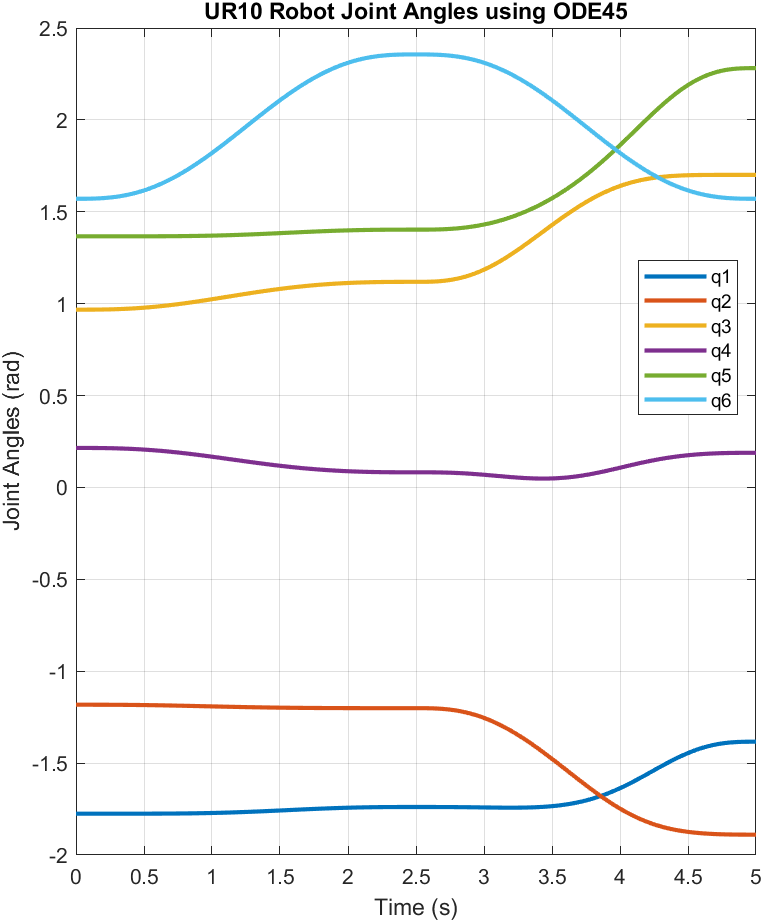
\includegraphics[width=0.9\linewidth]{plotsPartB/plot2_a_joint_position_ode.png}
        % \caption{Image 1}
    \end{minipage}
    \hfill
    \begin{minipage}{0.48\textwidth}
        \centering
        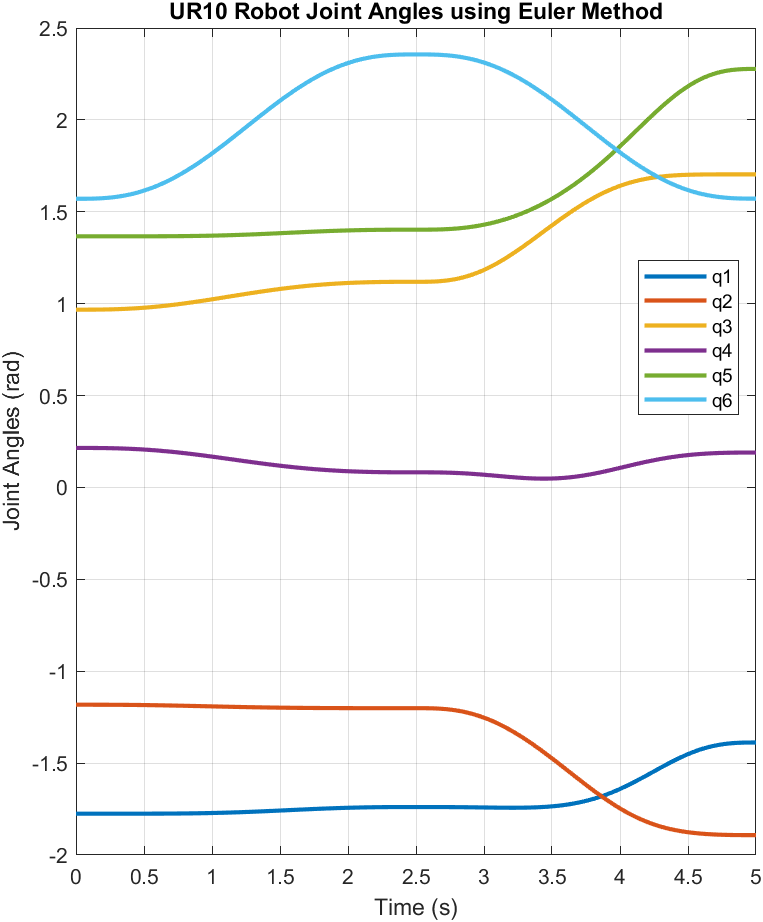
\includegraphics[width=0.9\linewidth]{plotsPartB/plot2_b_joint_position_euler.png}
        % \caption{Image 2}
    \end{minipage}
    
    \vspace{1em} % Space between rows
    
    \centering
    \begin{minipage}{0.98\textwidth}
        \centering
        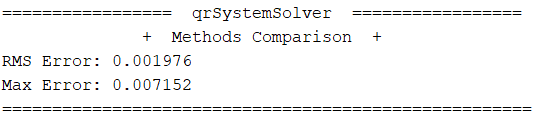
\includegraphics[width=0.5\linewidth]{plotsPartB/plot2_3_logs.png}
        % \caption{Image 1}
    \end{minipage}

    \caption{}
    \label{fig:qr}
\end{figure}


\begin{figure}[ht!]
    \centering
    \begin{minipage}{0.98\textwidth}
        \centering
        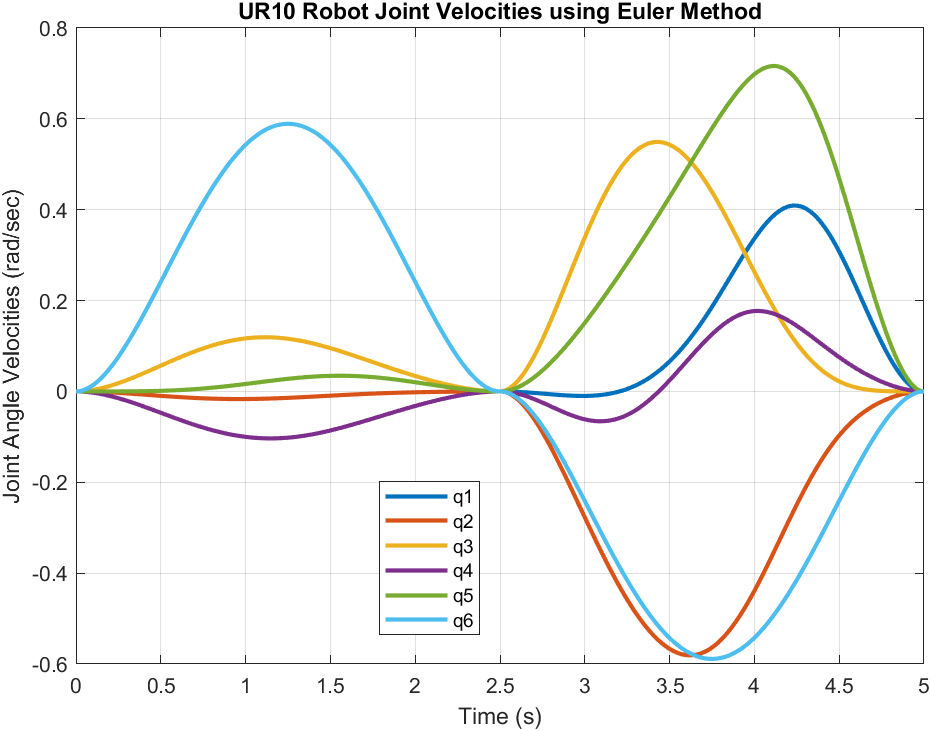
\includegraphics[width=0.5\linewidth]{plotsPartB/plot3_joint_velocity_euler.png}
        % \caption{Image 1}
    \end{minipage}
    
    \caption{}
    \label{fig:vel_joint}
\end{figure}

\textit{Σχόλιο}: Από τις γραφικές παραστάσεις των $q_r(t)$ και $\dot{q}_r(t)$ είναι εμφανές ότι οι θέσεις και οι ταχύτητες των αρθρώσεων είναι συνεχείς συναρτήσεις του χρόνου, (με μηδενικό ρυθμό μεταβολής στα αρχικά και τελικά σημεία της κίνησης).

Το Σχήμα~\ref{fig:Q_e} αναφέρεται στο άκρο (end effector) του ρομποτικού βραχίονα. 
Σε αυτό παρατίθενται οι γραφικές παραστάσεις της τροχιάς της θέσης του άκρου ως προς το πλαίσιο αναφοράς $\{0\}$ (κάτω δεξιά) και του προσανατολισμού αυτού (πάνω γραμμή) με χρήση Unit Quaternion, όπως εξηγήσαμε και από τις αντίστοιχες παραστάσεις του προηγούμενου τμήματος (για το πλαίσιο $\{H\}$).

\begin{figure}[ht!]
    \centering
    \begin{minipage}{0.48\textwidth}
        \centering
        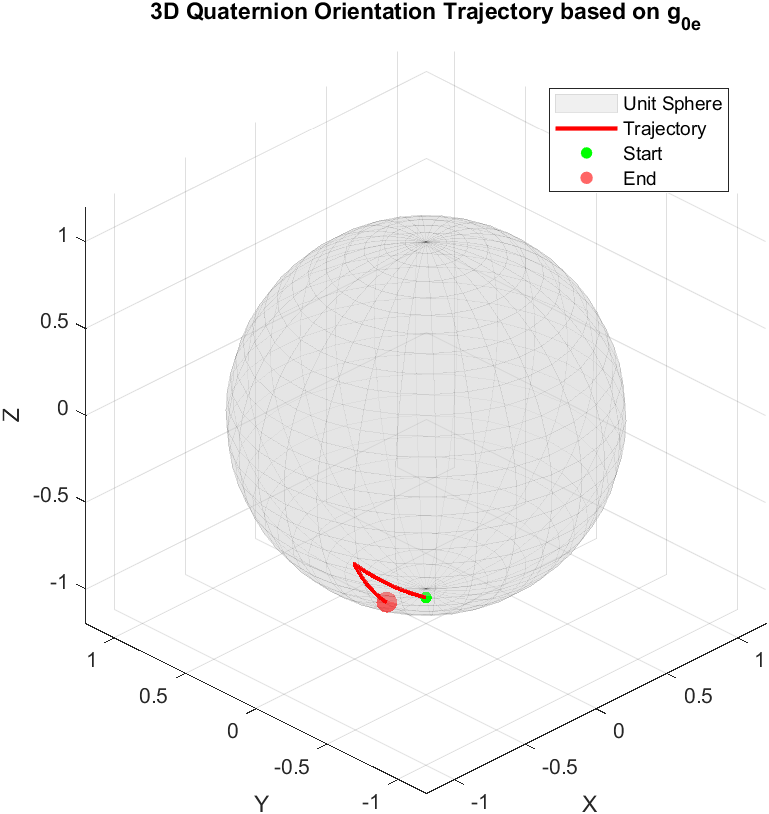
\includegraphics[width=0.8\linewidth]{plotsPartB/plot4_Q_sphere.png}
        % \caption{Image 1}
    \end{minipage}
    \hfill
    \begin{minipage}{0.48\textwidth}
        \centering
        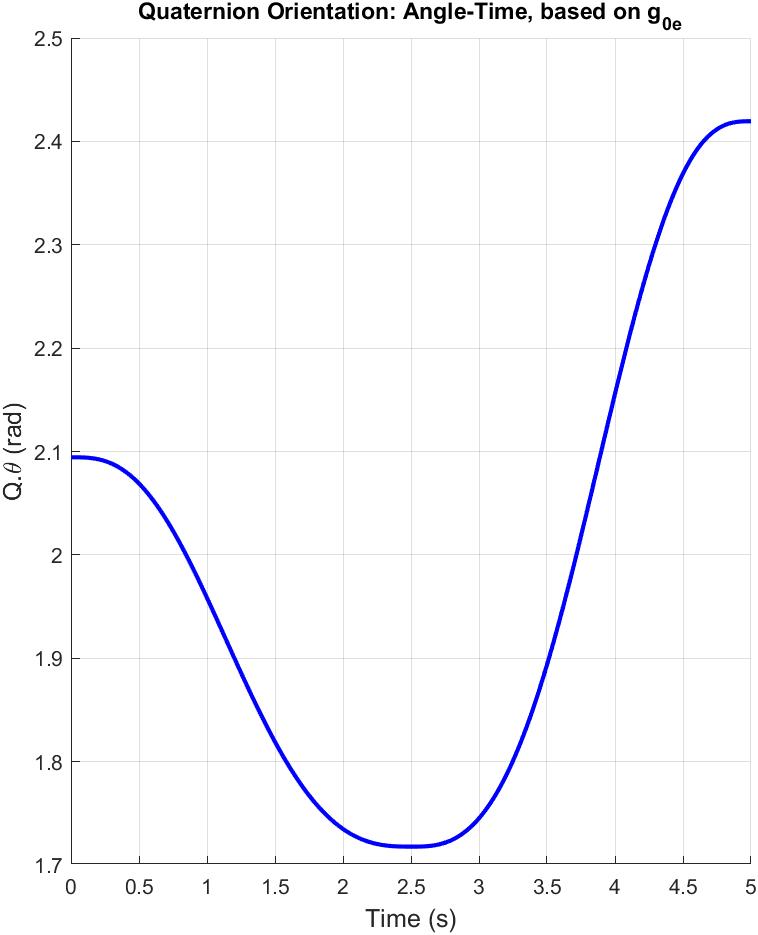
\includegraphics[width=0.7\linewidth]{plotsPartB/plot4_Q_theta.png}
        % \caption{Image 2}
    \end{minipage}
    
    \vspace{1em} % Space between rows
    
    \centering
    \begin{minipage}{0.48\textwidth}
        \centering
        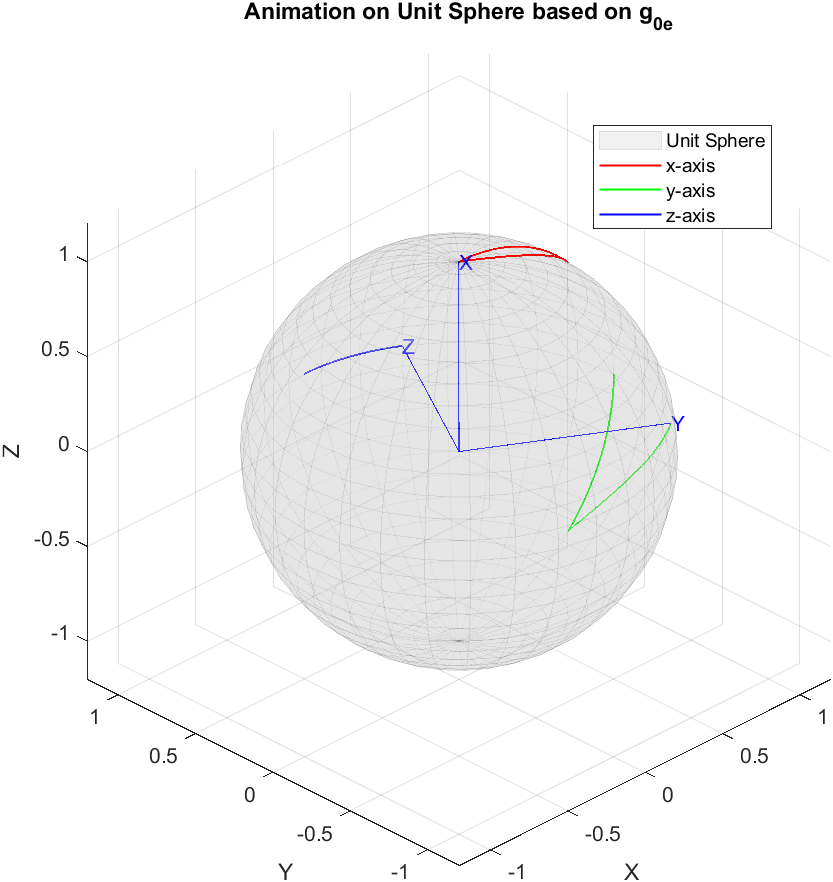
\includegraphics[width=0.8\linewidth]{plotsPartB/plot6_Q_animation.png}
        % \caption{Image 1}
    \end{minipage}
    \hfill
    \begin{minipage}{0.48\textwidth}
        \centering
        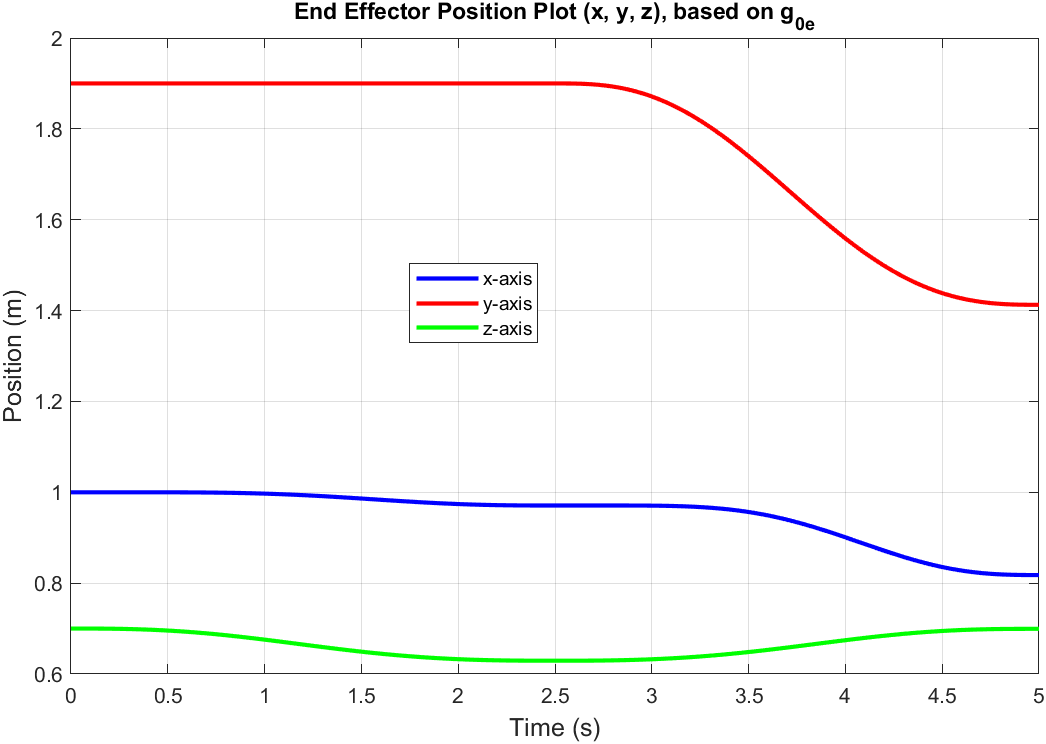
\includegraphics[width=1\linewidth]{plotsPartB/plot5_position_T0e.png}
        % \caption{Image 1}
    \end{minipage}
    
    \caption{}
    \label{fig:Q_e}
\end{figure}

Στην ανάλυσή μας, η λύση της ODE που βγάλαμε δεν είναι αναλυτική, δεν έχουμε δηλαδή τα $q_{r}(t), \forall t \in [t_0, t_f]$. 
Αντιθέτως, έχουμε λύσει το σύστημα με χρήση μιας αριθμητικής μεθόδου επίλυσης ODE, με βήμα $t_s = 0.01 \sec$.
Αυτό σημαίνει ότι περιμένουμε να υπάρχουν σφάλματα στα αποτελέσματά μας, που μπορεί να οδηγήσουν σε κίνηση του ρομποτικού βραχίονα που να είναι διαφορετική από την προβλεπόμενη. 

Για να μπορέσουμε να ελέγξουμε πόσο απέχουμε από την τροχιά που σχεδιάστηκε στο Τμήμα Α για το πόμολο της πόρτας $\{H\}$, 
σχεδιάζουμε τις γραφικές παραστάσεις του σχήματος \ref{fig:offset}. 
Αυτές αναφέρονται στην σχετική θέση του άκρου $\{e\}$, ως προς το το πλαίσιο $\{H\}$ (κάτω) αλλά και στον προσανατολισμό του $\{e\}$ ως προς το $\{H\}$.

\begin{figure}[ht!]
    \centering
    \begin{minipage}{0.48\textwidth}
        \centering
        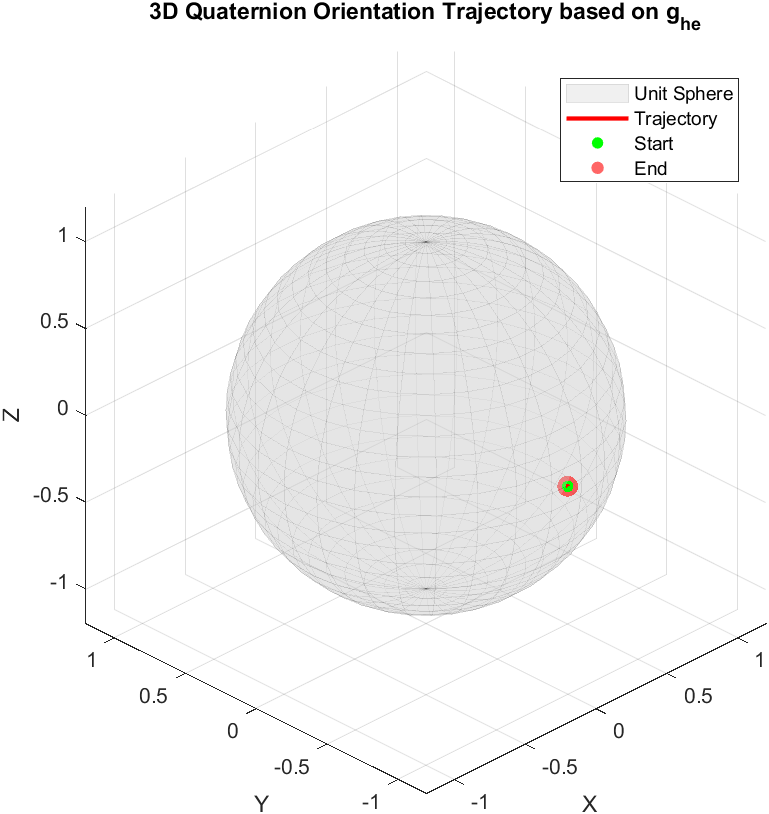
\includegraphics[width=0.8\linewidth]{plotsPartB/plot7_Q_sphere_The.png}
        % \caption{Image 1}
    \end{minipage}
    \hfill
    \begin{minipage}{0.48\textwidth}
        \centering
        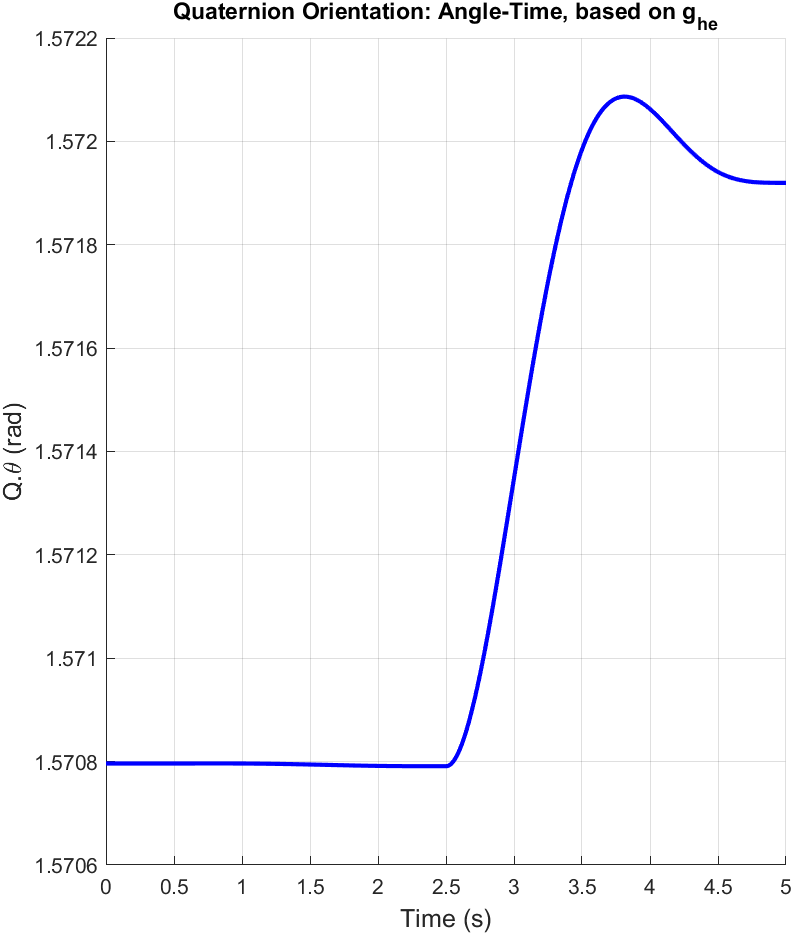
\includegraphics[width=0.7\linewidth]{plotsPartB/plot7_Q_theta_The.png}
        % \caption{Image 2}
    \end{minipage}
    
    \vspace{1em} % Space between rows
    
    \centering
    \begin{minipage}{0.48\textwidth}
        \centering
        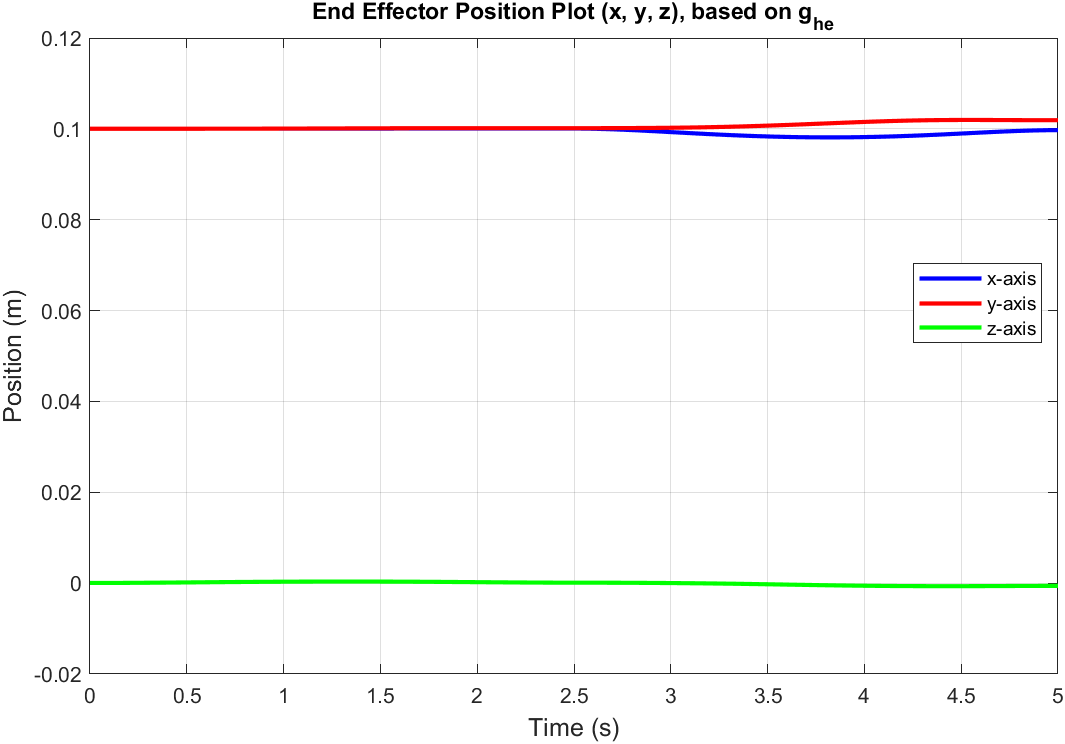
\includegraphics[width=0.8\linewidth]{plotsPartB/plot8_position_The.png}
        % \caption{Image 1}
    \end{minipage}
    
    \caption{}
    \label{fig:offset}
\end{figure}

Θεωρητικά, όπως αναφέραμε και στην μαθηματική ανάλυση, επειδή το άκρο του ρομπότ είναι προσαρτημένο πάνω στο πόμολο της πόρτας και η λαβή του είναι άκαμπτη θα έπρεπε η σχετική πόζα του άκρου ως προς το πόμολο της πόρτας να είναι σταθερή κάθε χρονική στιγμή.
Παρόλα αυτά, βλέπουμε από τις πάνω γραφικές παραστάσεις πως τόσο η θέση όσο και ο προσανατολισμός του άκρου έχουν μικρές διαφορές από το αναμενόμενο, λόγω των σφαλμάτων της χρήσης των αριθμητικών μεθόδων. 
Αυτή η διαφορά βέβαια, όπως φαίνεται, δεν είναι πολύ μεγάλη και εν τέλη η συνολική κίνηση θα διαφέρει ελάχιστα από αυτήν που σχεδιάστηκε στο Τμήμα Α. 

Στο τελευταίο section του κώδικα έχουμε ένα animation όλης της κίνησης. 
Παραθέτουμε παρακάτω το στιγμιότυπο για την τελική κατάσταση όπου $t = t_f$.
\begin{figure}[ht!]
    \centering
    \begin{minipage}{0.98\textwidth}
        \centering
        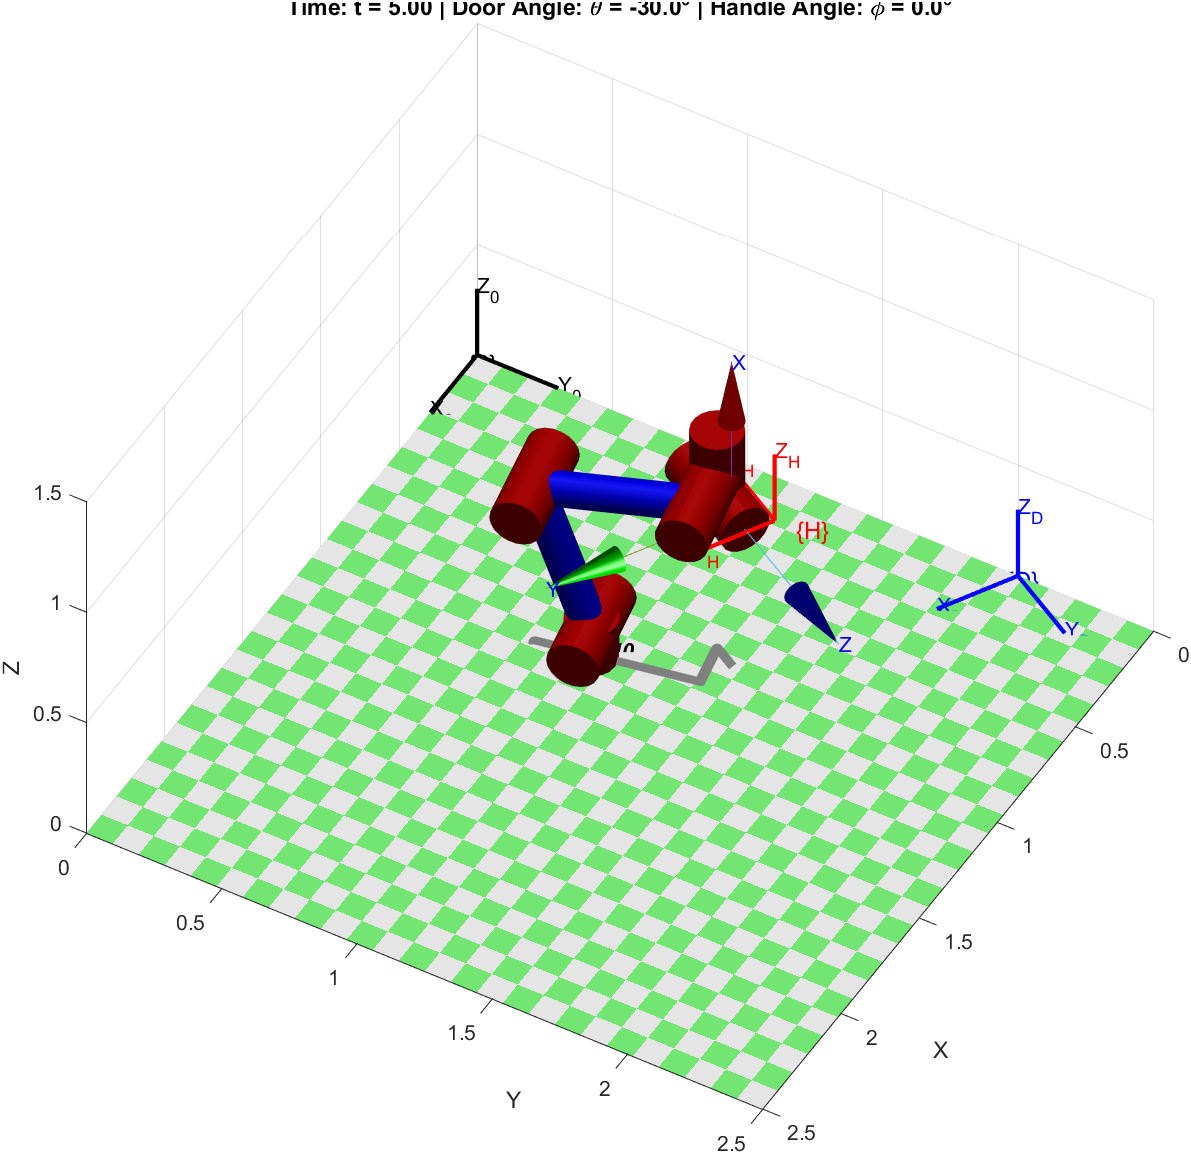
\includegraphics[width=0.6\linewidth]{plotsPartB/plot9_final_animation.png}
        % \caption{Image 1}
    \end{minipage}
    
    \caption{}
\end{figure}


\newpage

\end{document}
